% \usepackage{xcolor}
\usepackage[table,usenames,dvipsnames]{xcolor}

\usepackage{amsmath,amssymb,amsfonts}
\usepackage{graphicx}

\usepackage{nameref}

% For abbreviations, we use "acro" package, and mfirstuc to help capitalize long
% versions normally
\usepackage{mfirstuc}
\MFUhyphentrue % tell mfirstuc to capitalize hyphenated words

% Acronyms
\usepackage{acro}
% For one-offs,
% \DeclareAcronym{acronym}{short=short-version,long=long-version}

\newcommand{\newacr}[2]{\DeclareAcronym{#1}{short=\uppercase{#1},long=#2}}
\newcommand{\newacrs}[3]{\DeclareAcronym{#1}{short=#2,long=#3}}

% Alphabetically sorted list of acronyms
\newacr{aop}{Aspect-Oriented Programming}
\newacr{api}{Application Programming Interface}
\newacr{ast}{Abstract Syntax Tree}
\newacr{cms}{Content Management System}
\newacr{cpu}{Central Processing Unit}
\newacr{csv}{Comma-Separated Values}
\newacr{dsl}{Domain-Specific Language}
\newacr{ffi}{Foreign Function Interface}
\newacr{gui}{Graphical User Interface}
\newacr{html}{HyperText Markup Language}
\newacr{href}{Hypertext REFerence}
\newacr{ide}{Integrated Development Environment}
\newacr{json}{JavaScript Object Notation}
\newacr{jvm}{Java Virtual Machine}
\newacr{mop}{MetaObject Protocol}
\newacr{nasa}{National Aeronautics and Space Administration}
\newacr{pdf}{Portable Document Format}
\newacr{sst}{Skeleton Syntax Tree}
\newacr{wysiwyg}{What You See Is What You Get}

% Case Studies 
%   (note: I'm grouping these together and forcing "newacrs" usage, even when
%    seemingly unneeded because, otherwise, they won't group together at the 
%    bottom of the complete "acronyms" list.)
\newacrs{glassbr}{GlassBR}{Glass Breaking}
\newacrs{projectile}{Projectile}{Projectile}
\newacrs{sglpend}{SglPend}{Single Pendulum}
\newacrs{dblpend}{DblPend}{Double Pendulum}
\newacrs{gamephysics}{GamePhysics}{Game Physics}
\newacrs{hghc}{HGHC}{Heat Transfer Coefficients between Fuel and Cladding in Fuel Rods}
\newacrs{pdcontroller}{PDController}{Proportional Derivative Controller}
\newacrs{swhs}{SWHS}{Solar Water Heating System}
\newacrs{nopcm}{SWHSNoPCM}{Solar Water Heating System Without PCM}
\newacrs{ssp}{SSP}{Slope Stability analysis Program}


%------------------------------------------------------------------------------
%- Extra commands for more functionality -- in particular, capitalizing the
%- long form of acronyms.
%------------------------------------------------------------------------------

% Defining \ACL - to capitalize all words in an acronym
% Credits to: https://tex.stackexchange.com/a/257896
\NewDocumentCommand\ACF{sm}{%
  \begingroup
  \acsetup{uppercase/cmd=\ecapitalisewords}%
  \IfBooleanTF{#1}{\Acf*{#2}}{\Acf{#2}}%
  \endgroup
}

\NewDocumentCommand\ACFP{sm}{%
  \begingroup
  \acsetup{uppercase/cmd=\ecapitalisewords}%
  \IfBooleanTF{#1}{\Acfp*{#2}}{\Acfp{#2}}%
  \endgroup
}

\NewDocumentCommand\ACL{sm}{%
  \begingroup
  \acsetup{uppercase/cmd=\ecapitalisewords}%
  \IfBooleanTF{#1}{\Acl*{#2}}{\Acl{#2}}%
  \endgroup
}

\NewDocumentCommand\ACLP{sm}{%
  \begingroup
  \acsetup{uppercase/cmd=\ecapitalisewords}%
  \IfBooleanTF{#1}{\Aclp*{#2}}{\Aclp{#2}}%
  \endgroup
}


% General Assets
%------------------------------------------------------------------------------
% Code
%------------------------------------------------------------------------------

% Command based on: https://tex.stackexchange.com/questions/266811/define-a-new-command-with-parameters-inside-newcommand
\newcommand{\codeName}[1]{\expandafter\newcommand\csname #1\endcsname{\inlineHs{#1}}}

% Used for showing what the blue-highlighted text is, in the reading notes section
\codeName{ExampleText}

% Defines commands to be used in poster and thesis

\newcommand{\swebokScalDef}{This seems to define ``usability
    testing'' with elements of functional and recovery testing}
\newcommand{\swebokElasRef}{only cites a single source
    \textbf{that doesn't contain the words ``elasticity'' or ``elastic''}!}

% for assets/code/example.tex...
\newcommand{\exampleCode}{\begin{codeSnippet}{haskell}{``MultiDefinitions'' (MultiDefn) Definition}{exampleCode}{https://github.com/JacquesCarette/Drasil/blob/051b9881a6417e51e818c6673c5eab0f48bd5af2/code/drasil-theory/lib/Theory/Drasil/MultiDefn.hs\#L45-L56}
-- | 'MultiDefn's are QDefinition factories, used for showing one or more ways
--   we can define a QDefinition.
data MultiDefn e = MultiDefn{
  -- | UID
  _rUid :: UID,
  -- | Underlying quantity it defines.
  _qd :: QuantityDict,
  -- | Explanation of the different ways we can define a quantity.
  _rDesc :: Sentence,
  -- | All possible ways we can define the related quantity.
  _rvs :: NE.NonEmpty (DefiningExpr e)
}
\end{codeSnippet}
}
\newcommand{\refExampleCode}{\Cref{lst:exampleCode}}

% for assets/code/examplePseudocode.tex...
\newcommand{\examplePseudocode}{\begin{pseudocode}{haskell}{Broken QuantityDict Chunk Retriever}{examplePseudocode}
retrieveQD :: UID -> ChunkDB -> Maybe QuantityDict
retrieveQD u cdb = do
    (Chunk expectedQd) <- lookup u cdb
    pure expectedQd
\end{pseudocode}
}
\newcommand{\refExamplePseudocode}{\Cref{lst:examplePseudocode}}

% for assets/code/mainInvalidInputTest.tex...
\newcommand{\mainInvalidInputTest}{\begin{codeSnippet}{python}{Tests for main with an invalid input file}{mainInvalidInputTest}{https://github.com/samm82/Drasil/blob/sysTests/code/stable/projectile/projectile_c_p_nol_b_u_v_d/src/python/test/Control_test.py\#L29-L53}
  # from https://stackoverflow.com/questions/54071312/how-to-pass-command-line-argument-from-pytest-to-code
  ## \brief Tests main with invalid input file
  # \par Types of Testing:
  # Dynamic Black-Box (Behavioural) Testing
  # Boundary Conditions
  # Default, Empty, Blank, Null, Zero, and None
  # Invalid, Wrong, Incorrect, and Garbage Data
  # Logic Flow Testing
  @mark.parametrize("filename", invalid_value_input_files)
  @mark.xfail
  def test_main_invalid(monkeypatch, filename):
      # from https://stackoverflow.com/questions/10840533/most-pythonic-way-to-delete-a-file-which-may-not-exist
      try:
          remove(output_filename)
      except OSError as e: # this would be "except OSError, e:" before Python 2.6
          if e.errno != ENOENT: # no such file or directory
              raise # re-raise exception if a different error occurred


      assert not path.exists(output_filename)


      with monkeypatch.context() as m:
          m.setattr(sys, 'argv', ['Control.py', str(Path("test/test_input") / f"{filename}.txt")])
          Control.main()
      
      assert not path.exists(output_filename)
\end{codeSnippet}
}
\newcommand{\refMainInvalidInputTest}{\Cref{lst:mainInvalidInputTest}}

% for assets/code/projManualViolationReq.tex...
\newcommand{\projManualViolationReq}{\begin{codeSnippet}{haskell}{\acs{projectile}'s manually created requirement for constraint violation behaviour}{projManualViolationReq}{https://github.com/JacquesCarette/Drasil/blob/afb6fb752b8364d2807ced7fc0c1dd6c6aba52b2/code/drasil-example/projectile/lib/Drasil/Projectile/Requirements.hs\#L31-L34}
verifyParamsDesc = foldlSent [S "Check the entered", plural inValue,
    S "to ensure that they do not exceed the" +:+. namedRef (datCon [] []) (plural datumConstraint),
    S "If any of the", plural inValue, S "are out of bounds" `sC`
    S "an", phrase errMsg, S "is displayed" `S.andThe` plural calculation, S "stop"]
\end{codeSnippet}
}
\newcommand{\refProjManualViolationReq}{\Cref{lst:projManualViolationReq}}

% for assets/code/projViolationChoice.tex...
\newcommand{\projViolationChoice}{\begin{codeSnippet}{haskell}{\acs{projectile}'s choice for constraint violation behaviour in code}{projViolationChoice}{https://github.com/JacquesCarette/Drasil/blob/afb6fb752b8364d2807ced7fc0c1dd6c6aba52b2/code/drasil-example/projectile/lib/Drasil/Projectile/Choices.hs\#L120}
    srsConstraints = makeConstraints Warning Warning,
\end{codeSnippet}
}
\newcommand{\refProjViolationChoice}{\Cref{lst:projViolationChoice}}

%------------------------------------------------------------------------------
% Graphs
%------------------------------------------------------------------------------

% Organization of files

\newcommand{\parChdGraphs}{
    % Only top or bottom to comply with IEEE guidelines
    \begin{figure}[bt!]
        \centering
        \begin{subfigure}[b]{\linewidth}
            \centering
            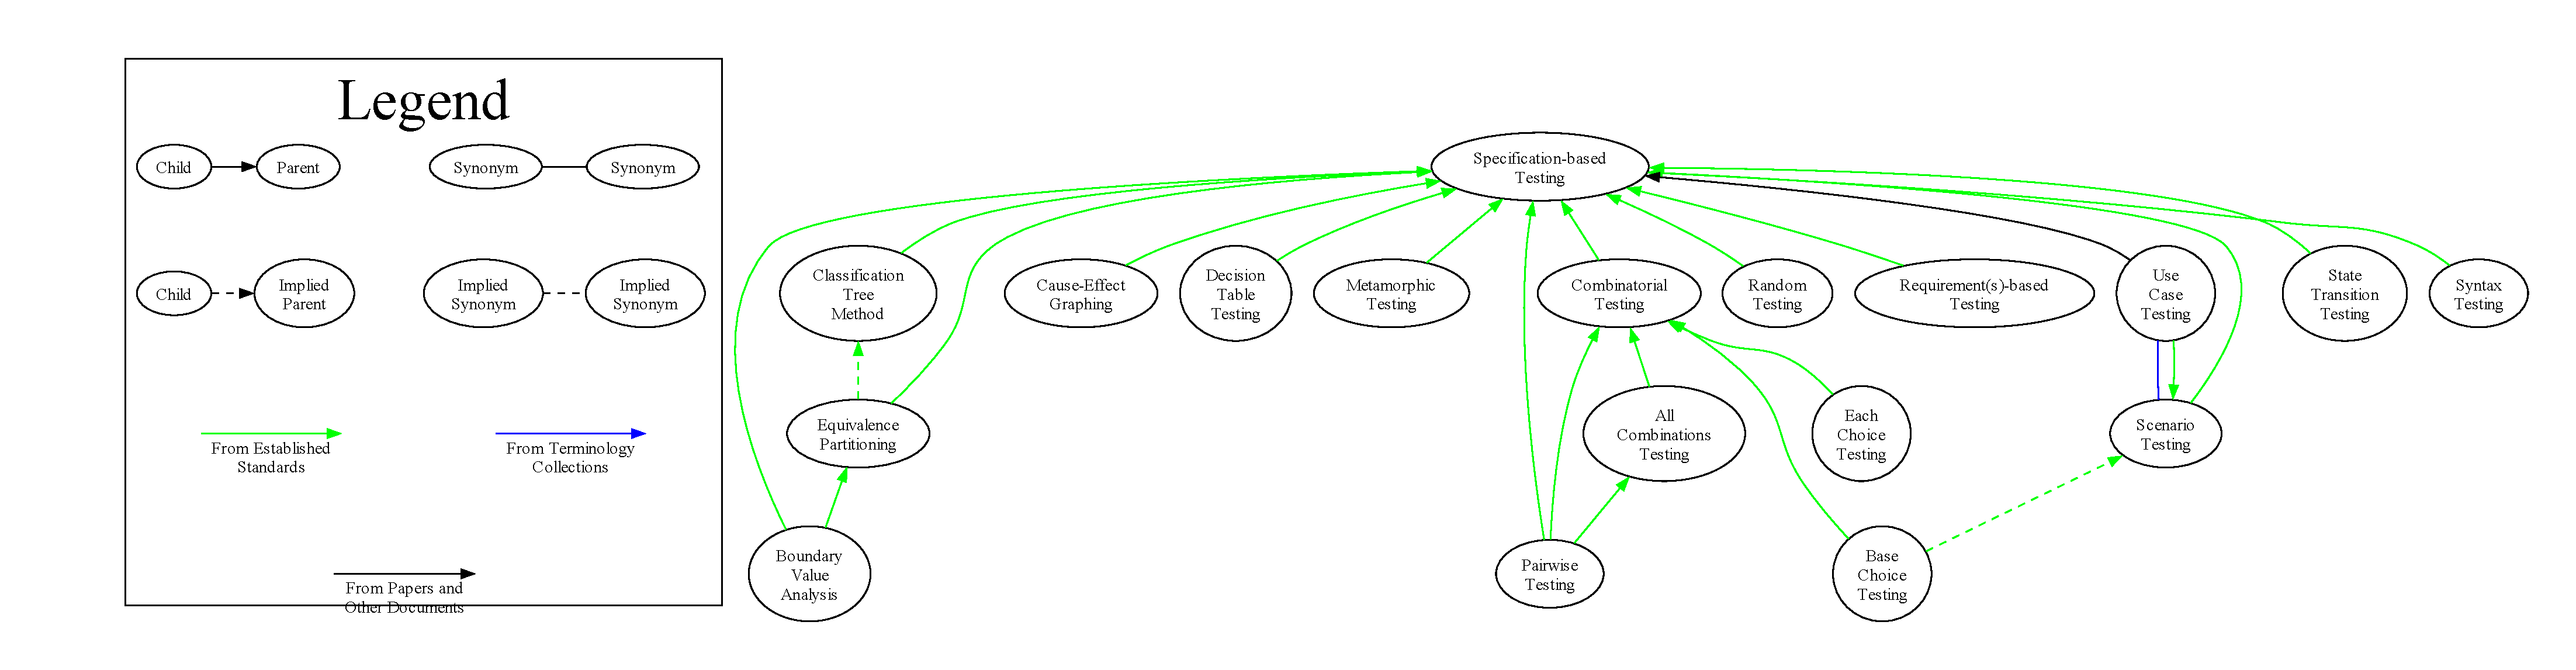
\includegraphics[width=\linewidth]{assets/graphs/specBasedGraph.pdf}
            \caption{``Superset'' relations.}
            \label{fig:specBasedGraph}
        \end{subfigure}
        \begin{subfigure}[t]{.45\linewidth}
            \centering
            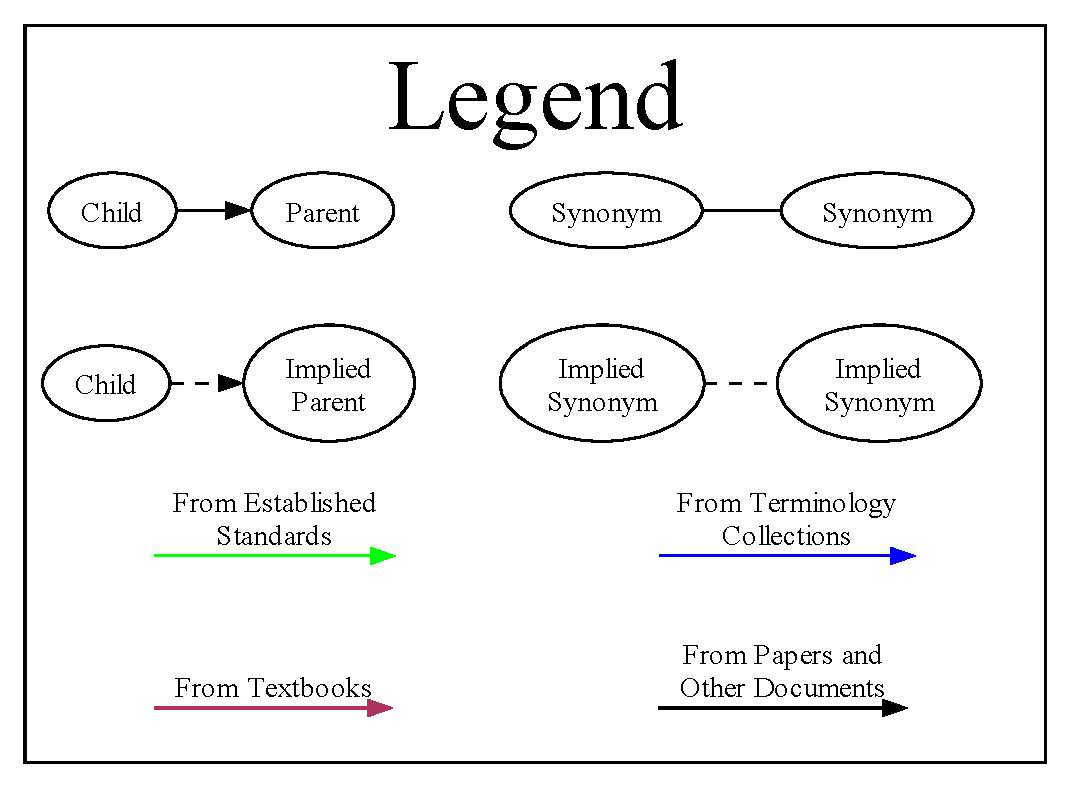
\includegraphics[width=\linewidth]{assets/graphs/parChdLegend.pdf}
        \end{subfigure}
        \begin{subfigure}[t]{.5\linewidth}
            \centering
            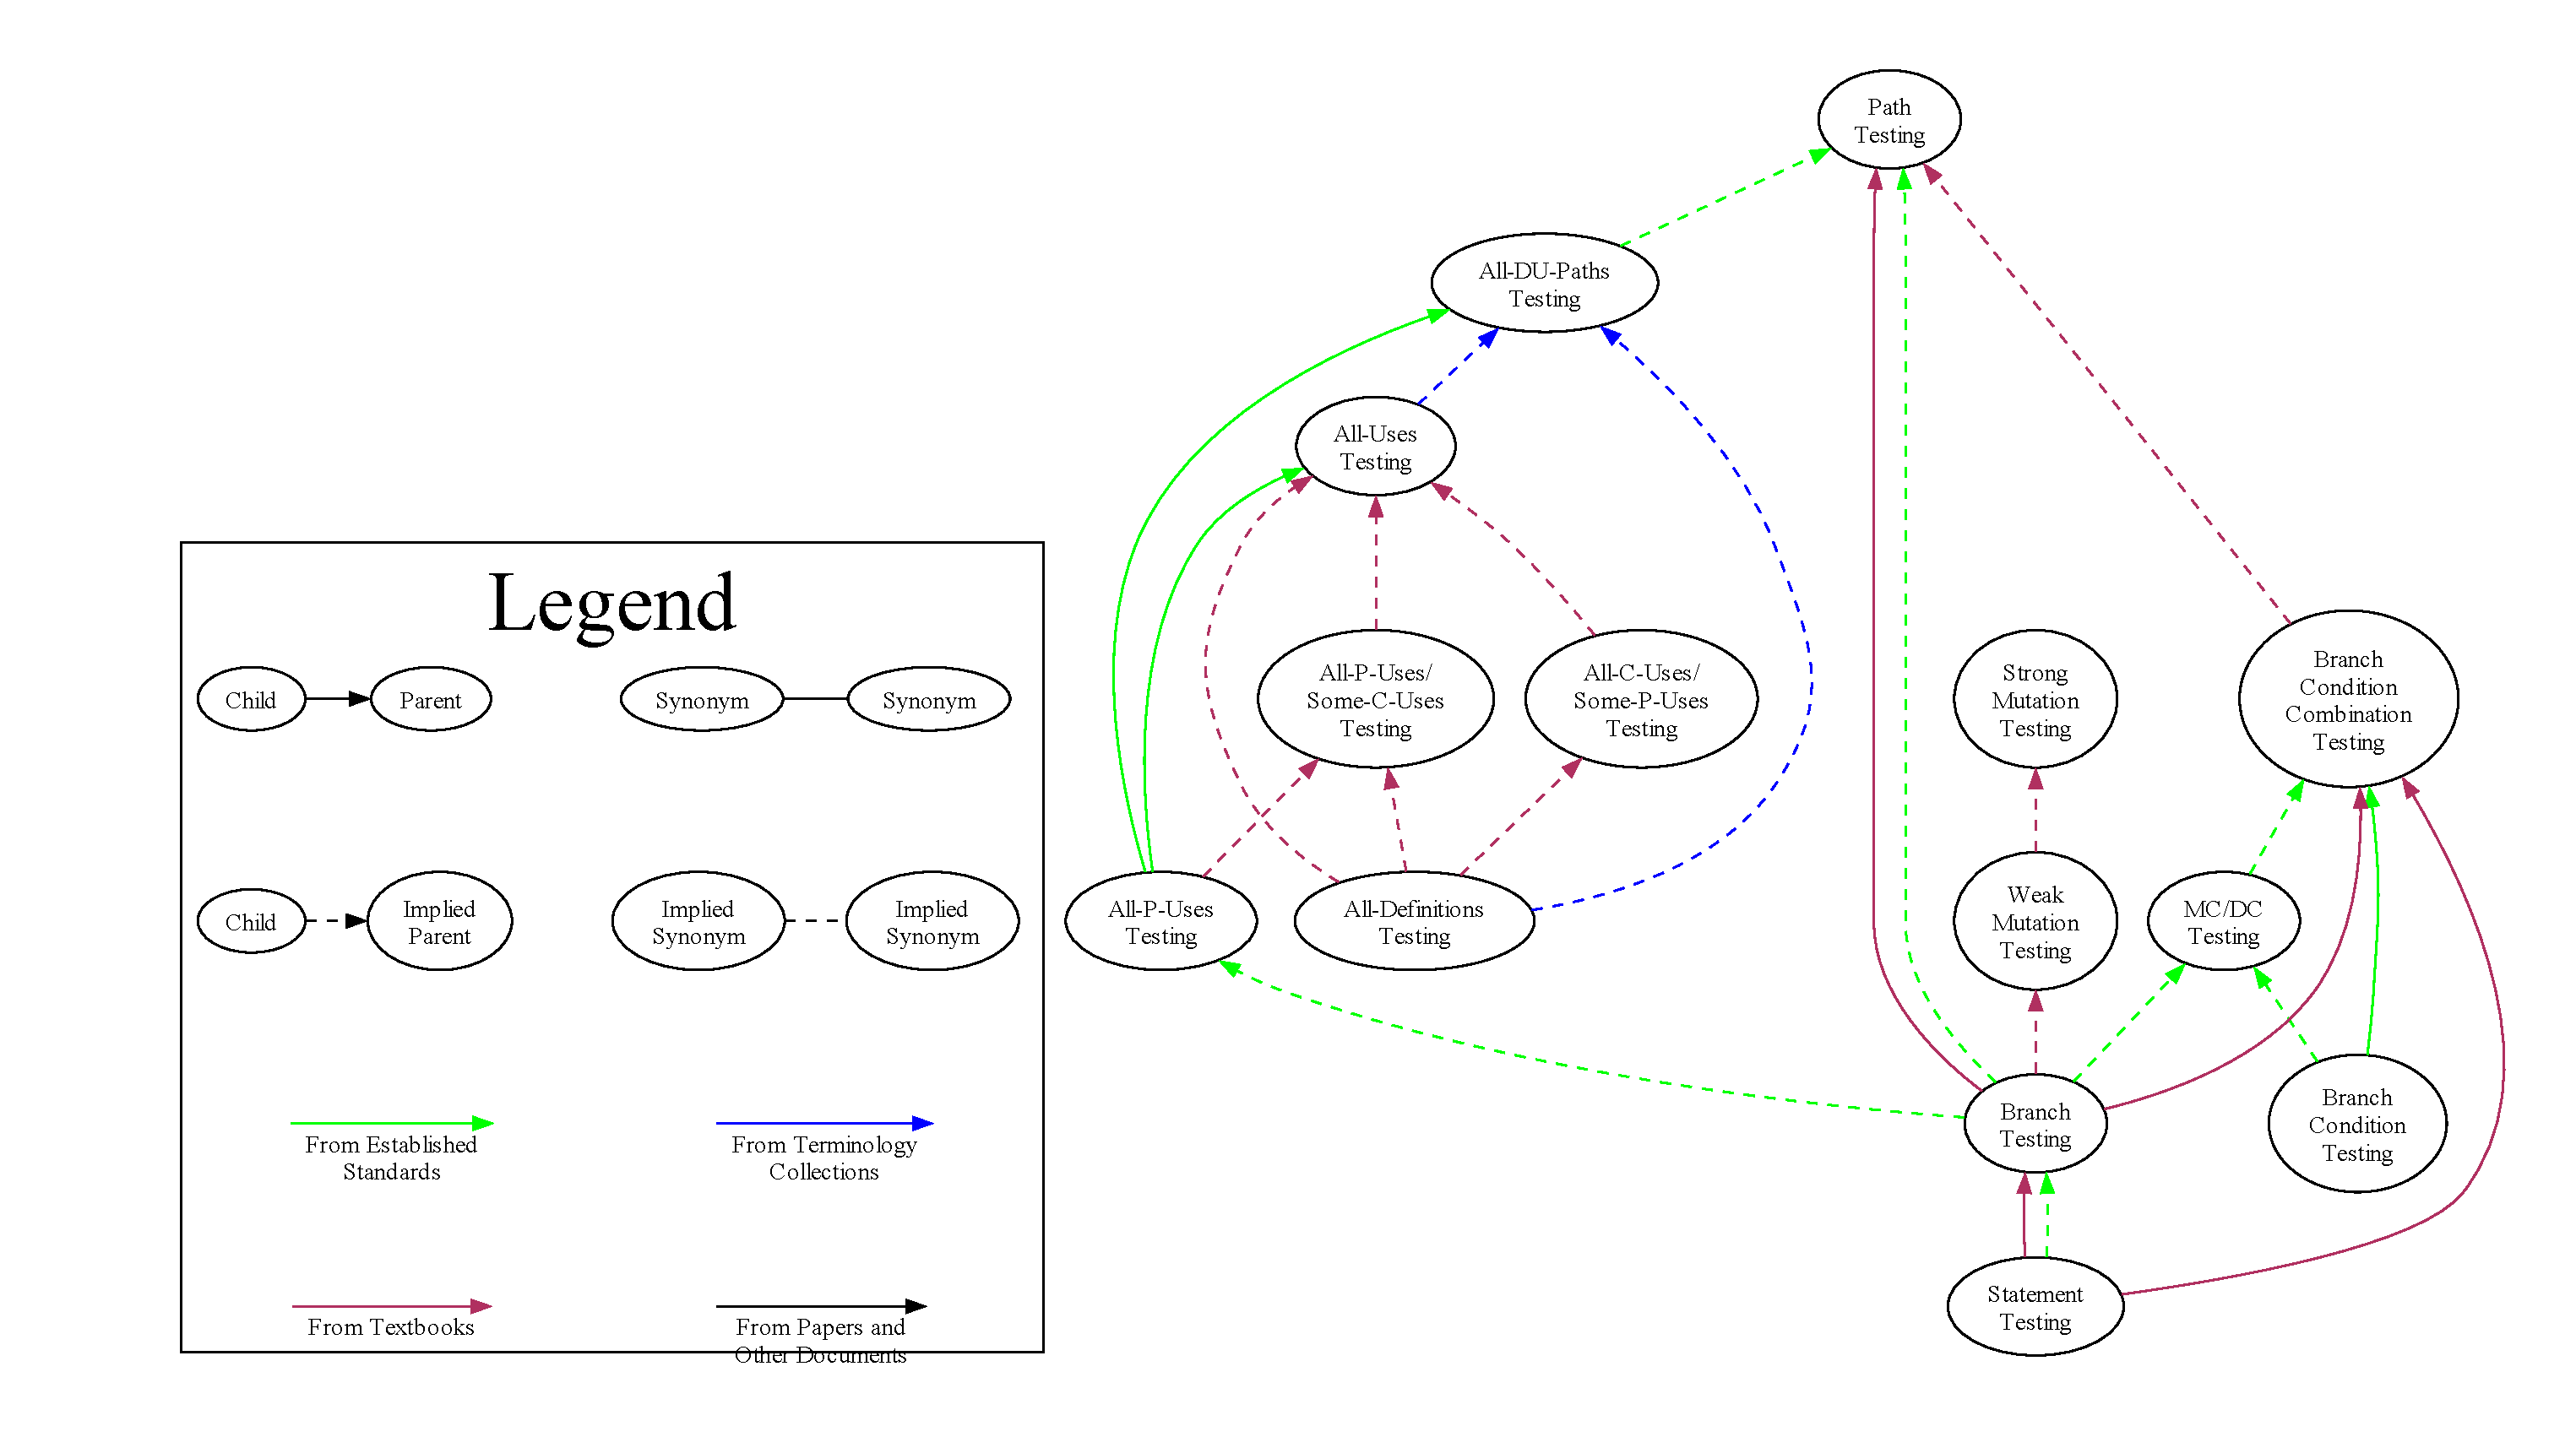
\includegraphics[width=\linewidth]{assets/graphs/subsumesGraph.pdf}
            \caption{``Subsume'' relations.}
            \label{fig:subsumesGraph}
        \end{subfigure}
        \caption{Graphs of different classes of \hyperref[par-chd-rels]{parent-child relations}.}
        \label{fig:parChdGraphs}
    \end{figure}
}

\newcommand{\ExampleGraph}{
    \begin{figure*}
        \begin{subfigure}[b]{0.3\linewidth}
            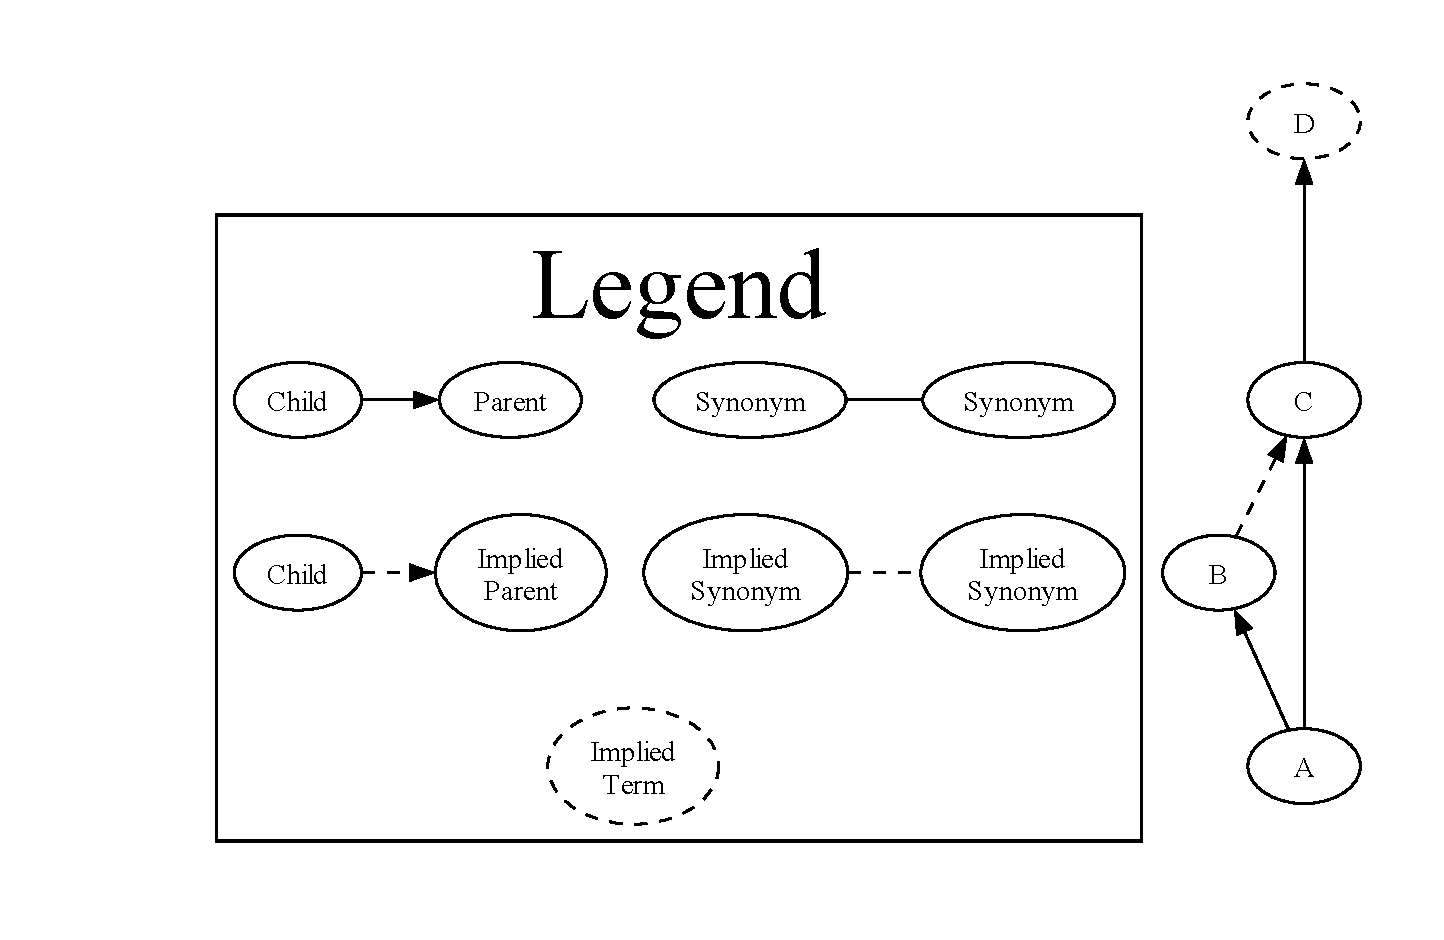
\includegraphics[width=\linewidth]{assets/graphs/ExampleGlossaryGraph.pdf}
            \caption{Graph from \Cref{tab:exampleGlossary}.}
            \label{fig:exampleGraph}
        \end{subfigure}
        \centering
        \begin{subfigure}[b]{0.675\linewidth}
            \centering
            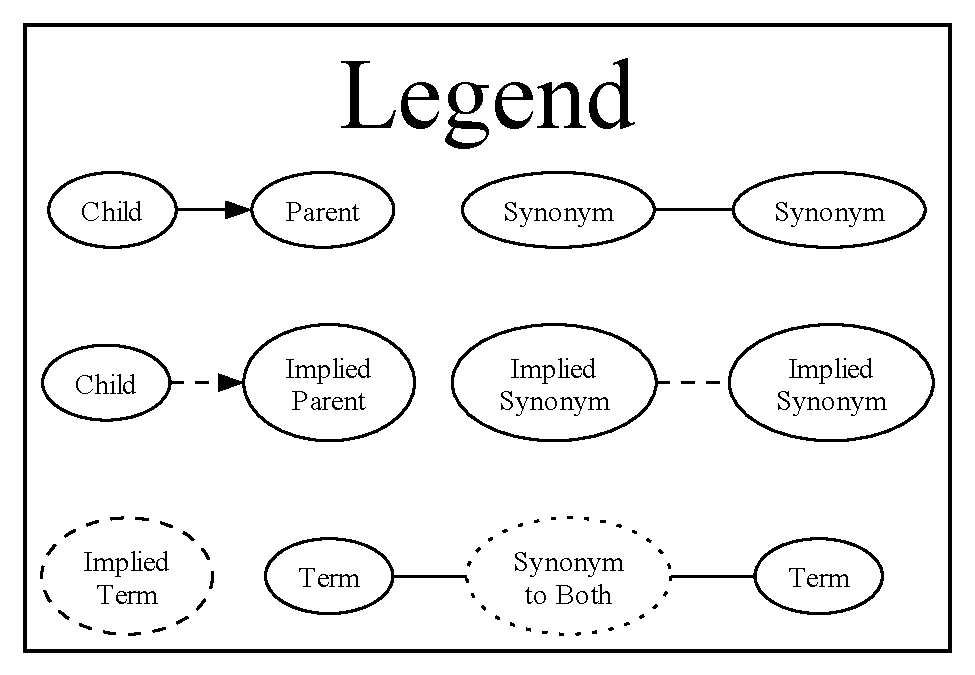
\includegraphics[width=0.8\linewidth]{assets/graphs/manual/manualLegendNonSolidTerms.pdf}
            \hspace{5cm}\begin{subfigure}[t]{0.475\linewidth}
                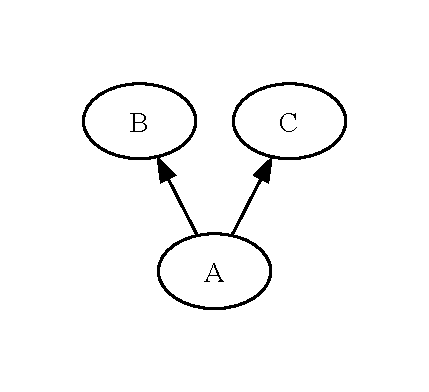
\includegraphics[width=1.1\linewidth]{assets/graphs/rigidExampleGlossaryGraph.pdf}
                \caption{Rigid graph from\\\Cref{tab:exampleGlossary}.}
                \label{fig:rigidExampleGraph}
            \end{subfigure}
            \begin{subfigure}[t]{0.475\linewidth}
                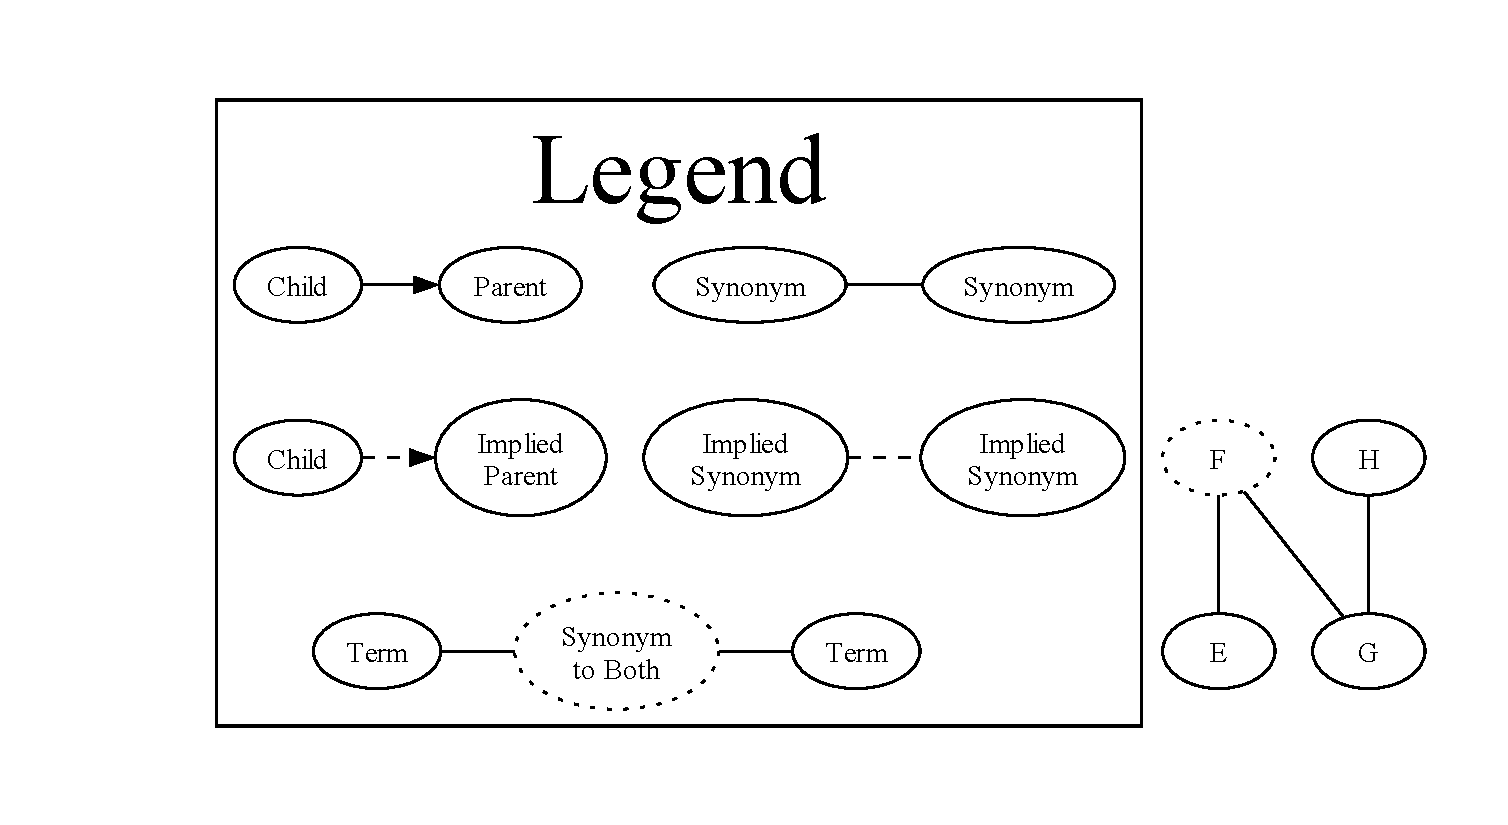
\includegraphics[width=1.1\linewidth]{assets/graphs/SynExampleGlossaryGraph.pdf}
                \caption{Graph from \Cref{tab:synExampleGlossary}.}
                \label{fig:synExampleGraph}
            \end{subfigure}
        \end{subfigure}
        \begin{subfigure}[t]{0.25\linewidth}
            \centering
            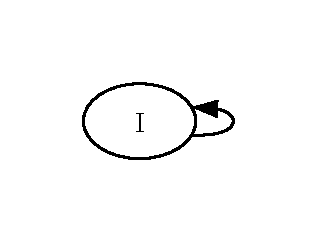
\includegraphics[width=1.2\linewidth]{assets/graphs/SelfExampleGlossaryGraph.pdf}
            \caption{Self-loop graph.}
            \label{fig:selfExampleGraph}
        \end{subfigure}
        \hfill
        \begin{subfigure}[t]{0.425\linewidth}
            \centering
            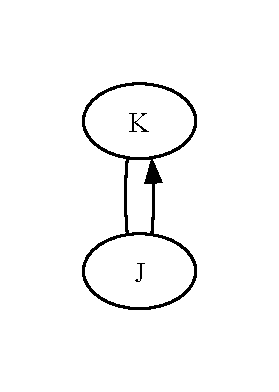
\includegraphics[width=0.6\linewidth]{assets/graphs/ParSynExampleGlossaryGraph.pdf}
            \caption{Graph of a pair of terms with a \hyperref[par-chd-rels]{parent-child} \emph{and} synonym relation.}
            \label{fig:parSynExampleGraph}
        \end{subfigure}
        \hfill
        \begin{subfigure}[t]{0.25\linewidth}
            \centering
            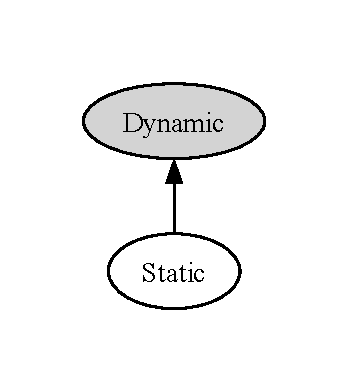
\includegraphics[width=1.4\linewidth]{assets/graphs/StaticExampleGlossaryGraph.pdf}
            \caption{Static graph.}
            \label{fig:staticExampleGraph}
        \end{subfigure}
        \caption{Example generated graphs.}
        \label{fig:exampleGraphs}
    \end{figure*}
}

\newcommand{\recoveryGraphs}{
    % Only top or bottom to comply with IEEE guidelines
    \begin{figure}[bt!]
        \centering
        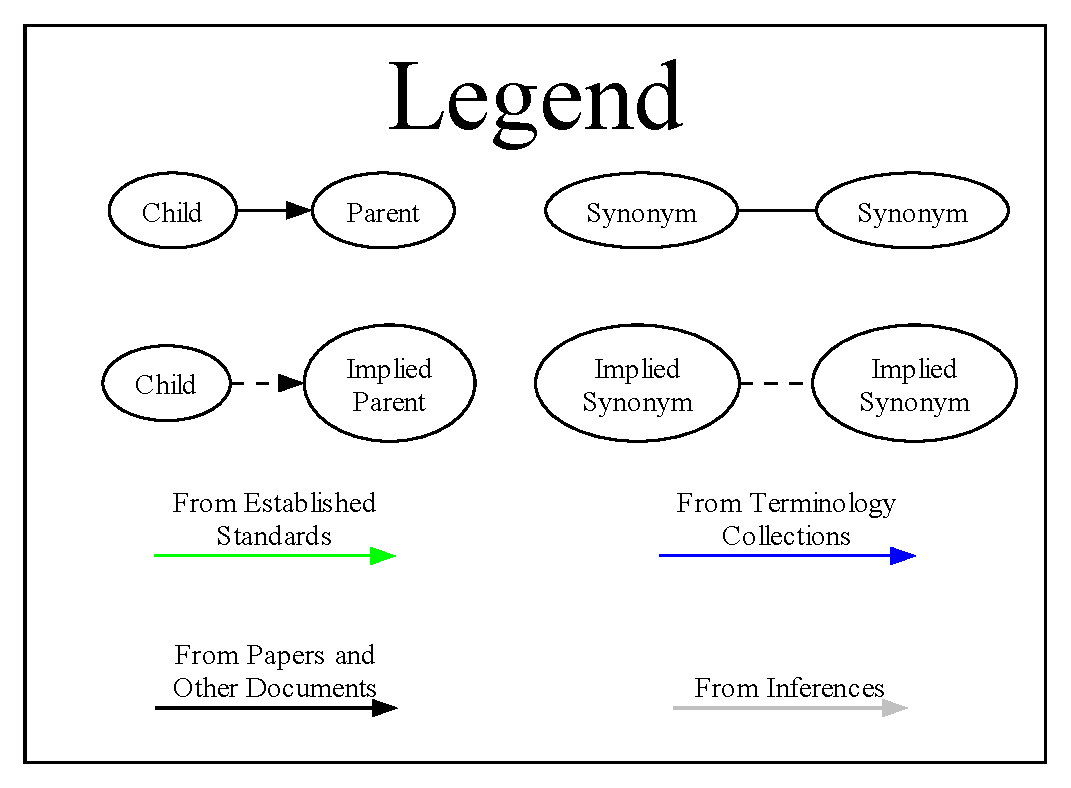
\includegraphics[width=\linewidth]{assets/graphs/recoveryLegend.pdf}
        \begin{subfigure}[b]{.55\linewidth}
            \centering
            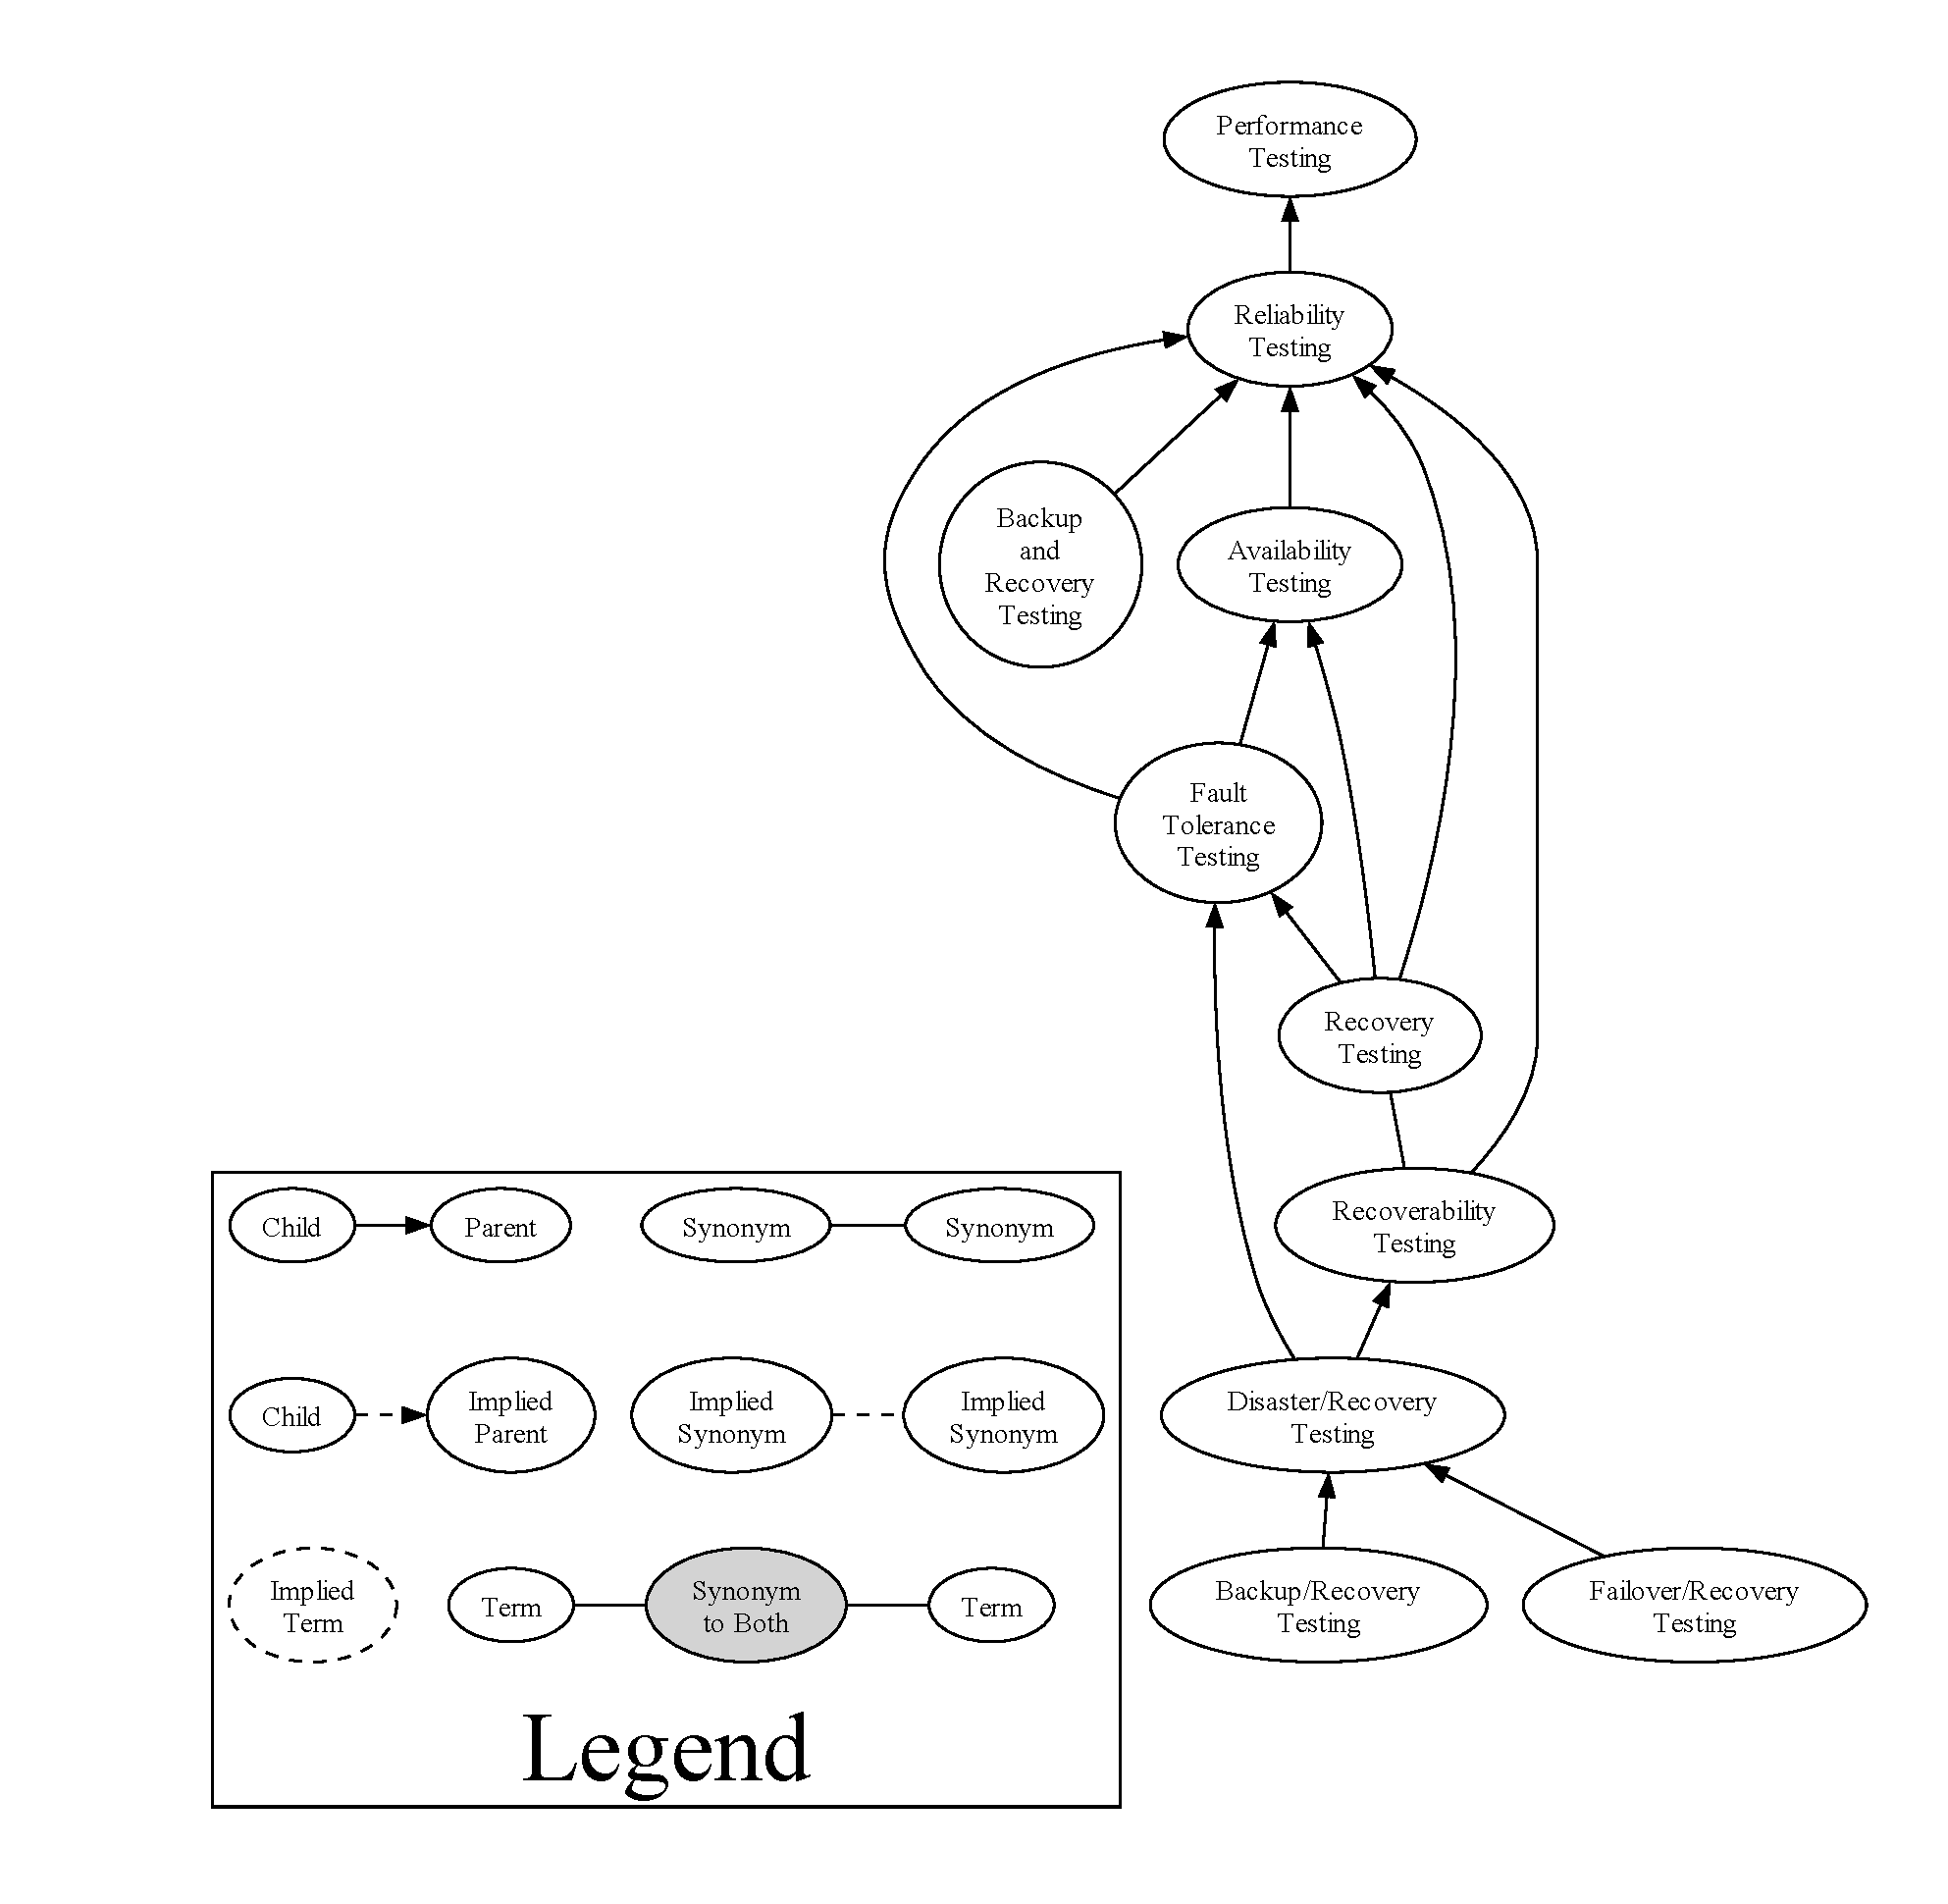
\includegraphics[width=\linewidth]{assets/graphs/recoveryGraph.pdf}
            \caption{Graph of current relations.}
            \label{fig:recovery-graph-current}
        \end{subfigure}
        \begin{subfigure}[b]{.4\linewidth}
            \centering
            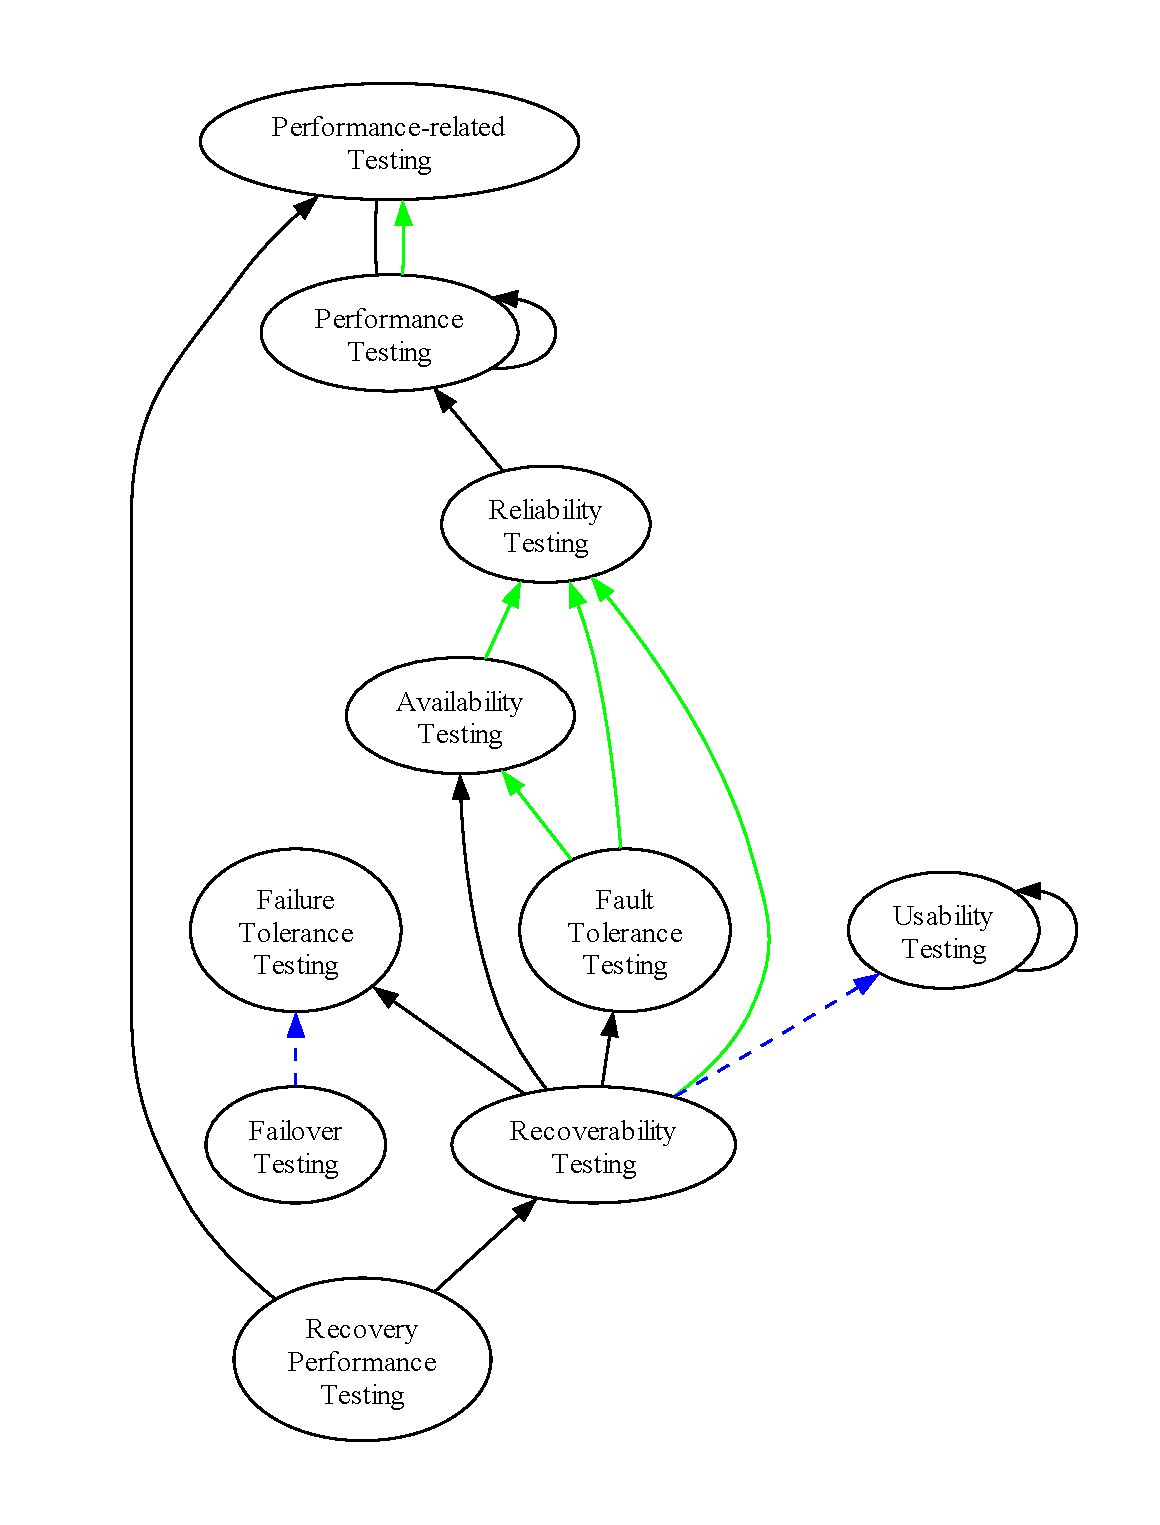
\includegraphics[width=\linewidth]{assets/graphs/recoveryProposedGraph.pdf}
            \caption{Graph of proposed relations.}
            \label{fig:recovery-graph-proposed}
        \end{subfigure}
        \caption{Graphs of relations between terms related to recovery testing.}
        \label{fig:recoveryGraphs}
    \end{figure}
}

\newcommand{\scalGraphs}{
    % Only top or bottom to comply with IEEE guidelines
    \begin{figure}[bt!]
        \centering
        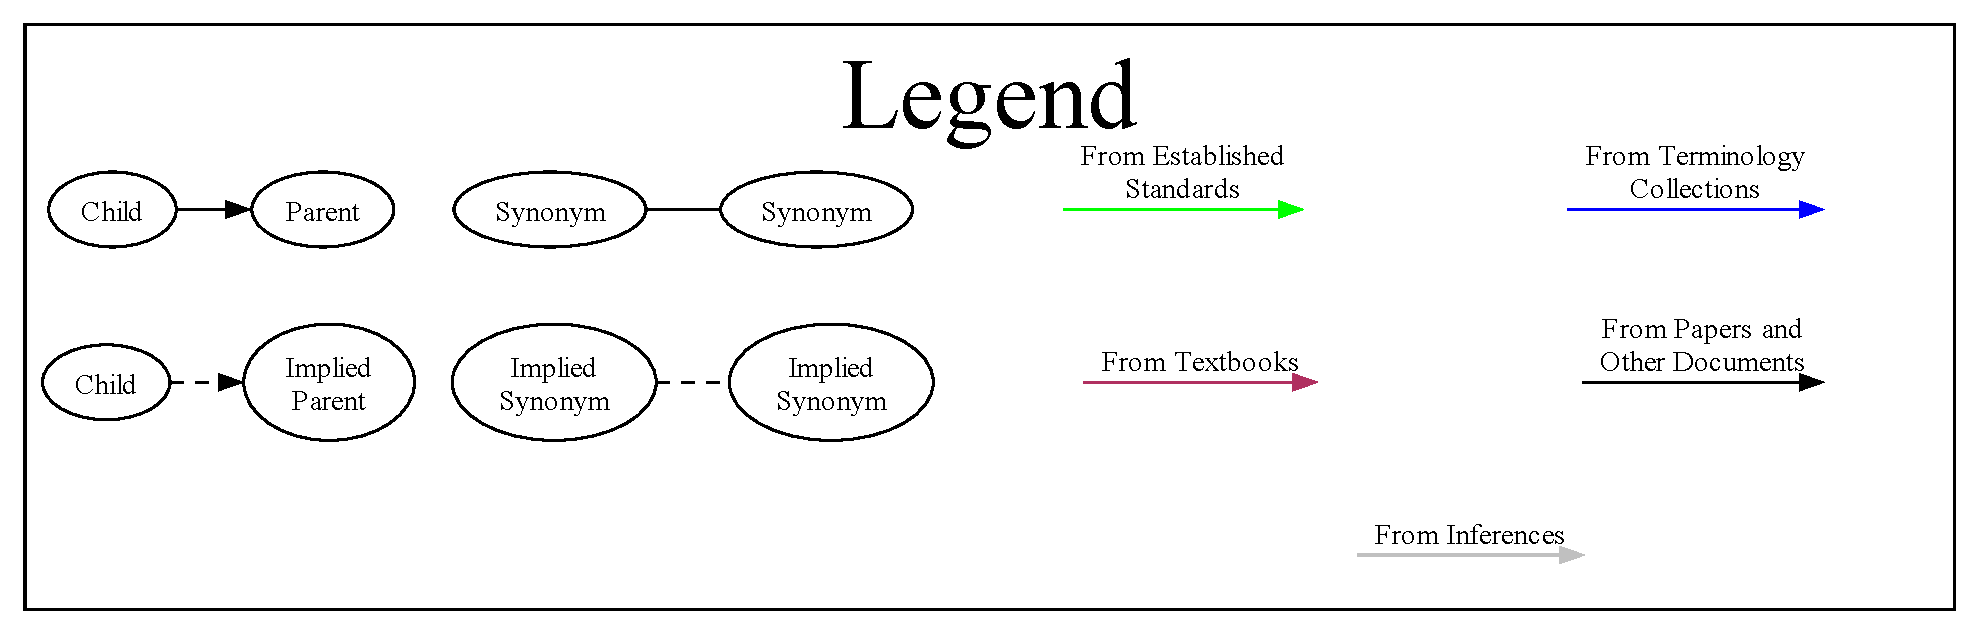
\includegraphics[width=\linewidth]{assets/graphs/scalabilityLegend.pdf}
        \begin{subfigure}[b]{.475\linewidth}
            \centering
            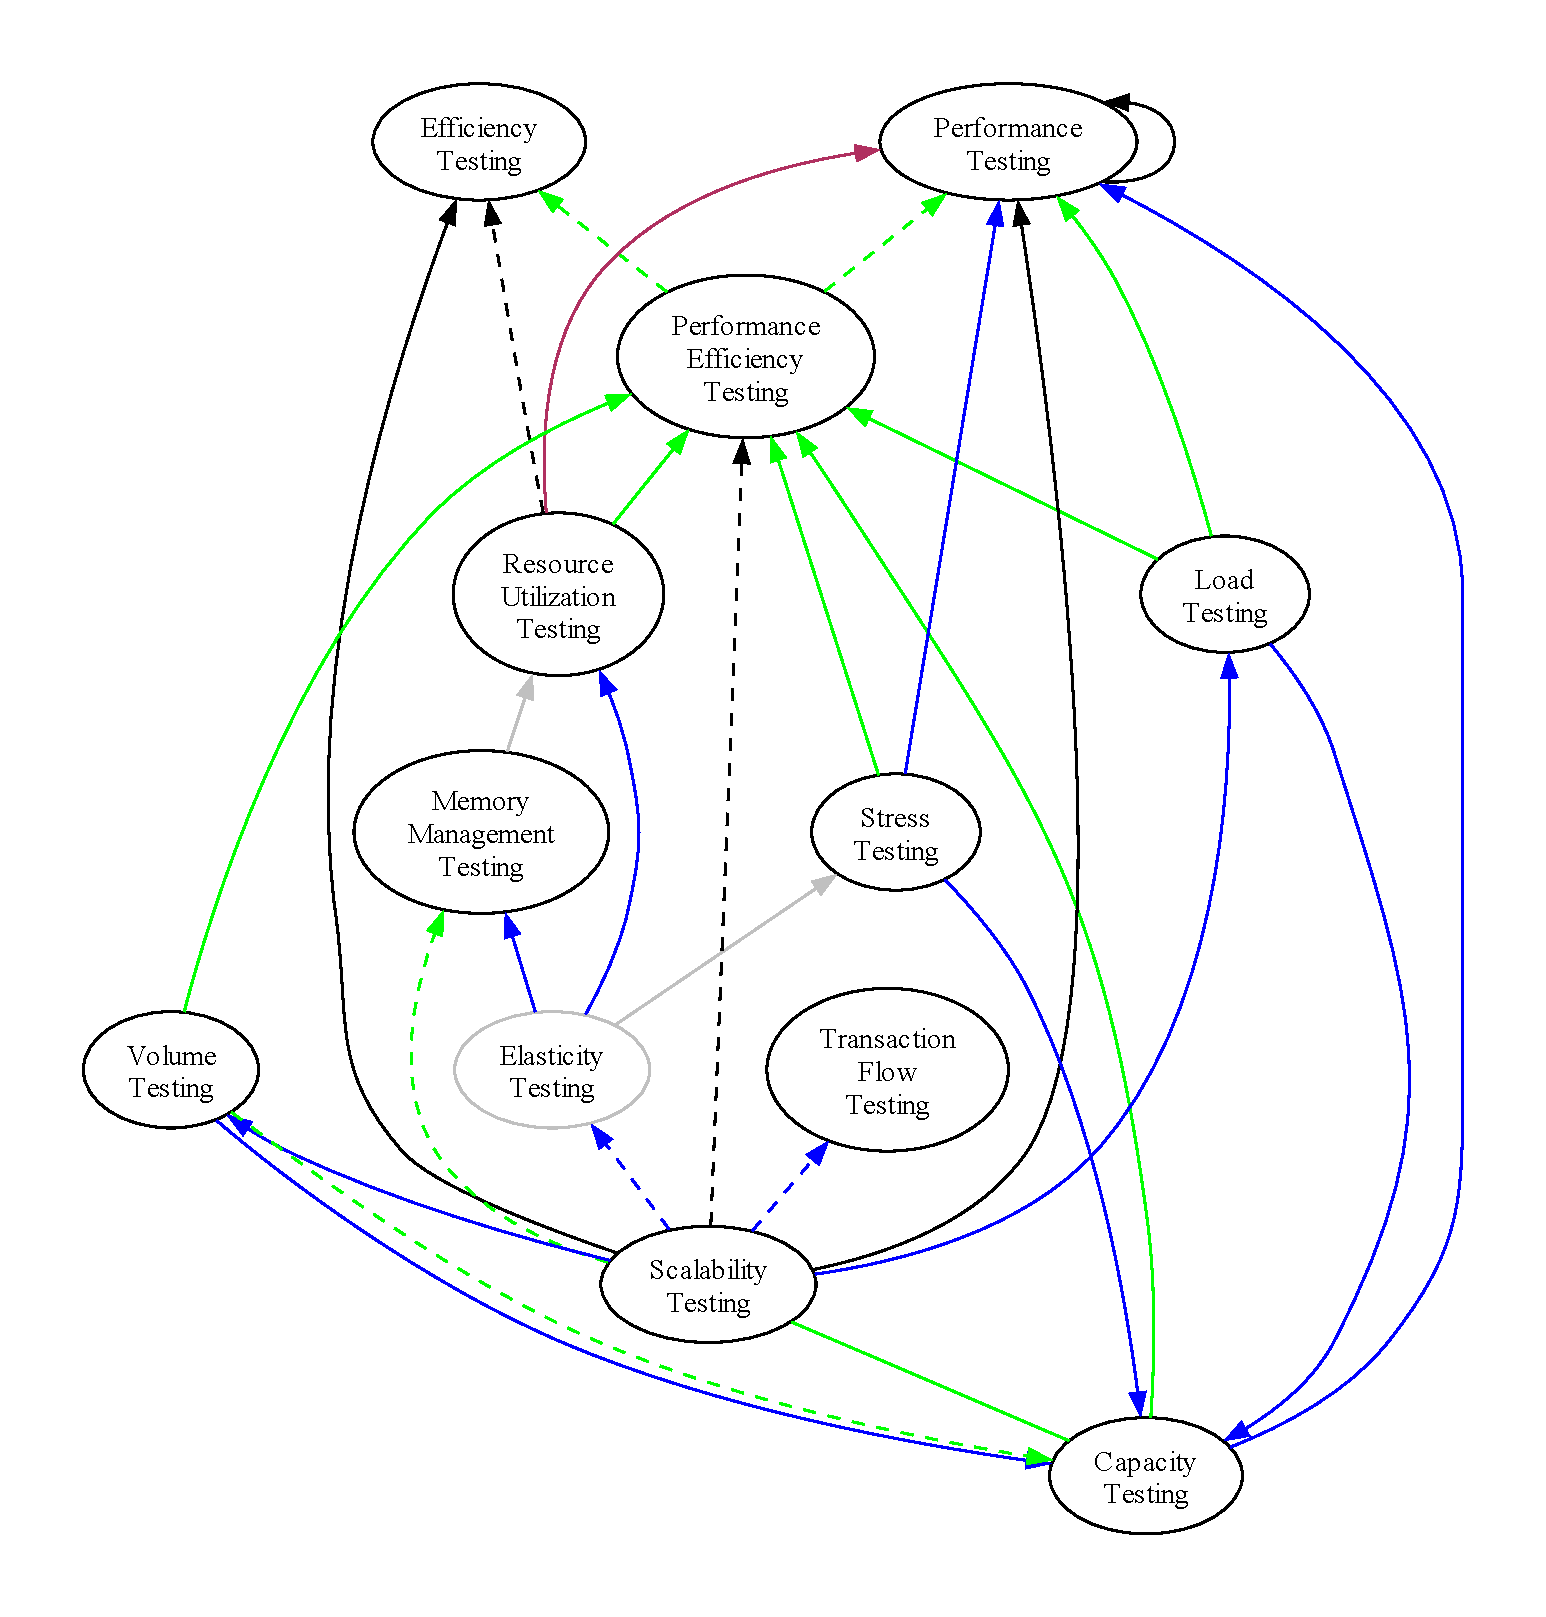
\includegraphics[width=\linewidth]{assets/graphs/scalabilityGraph.pdf}
            \caption{Graph of current relations.}
            \label{fig:scal-graph-current}
        \end{subfigure}
        \begin{subfigure}[b]{.475\linewidth}
            \centering
            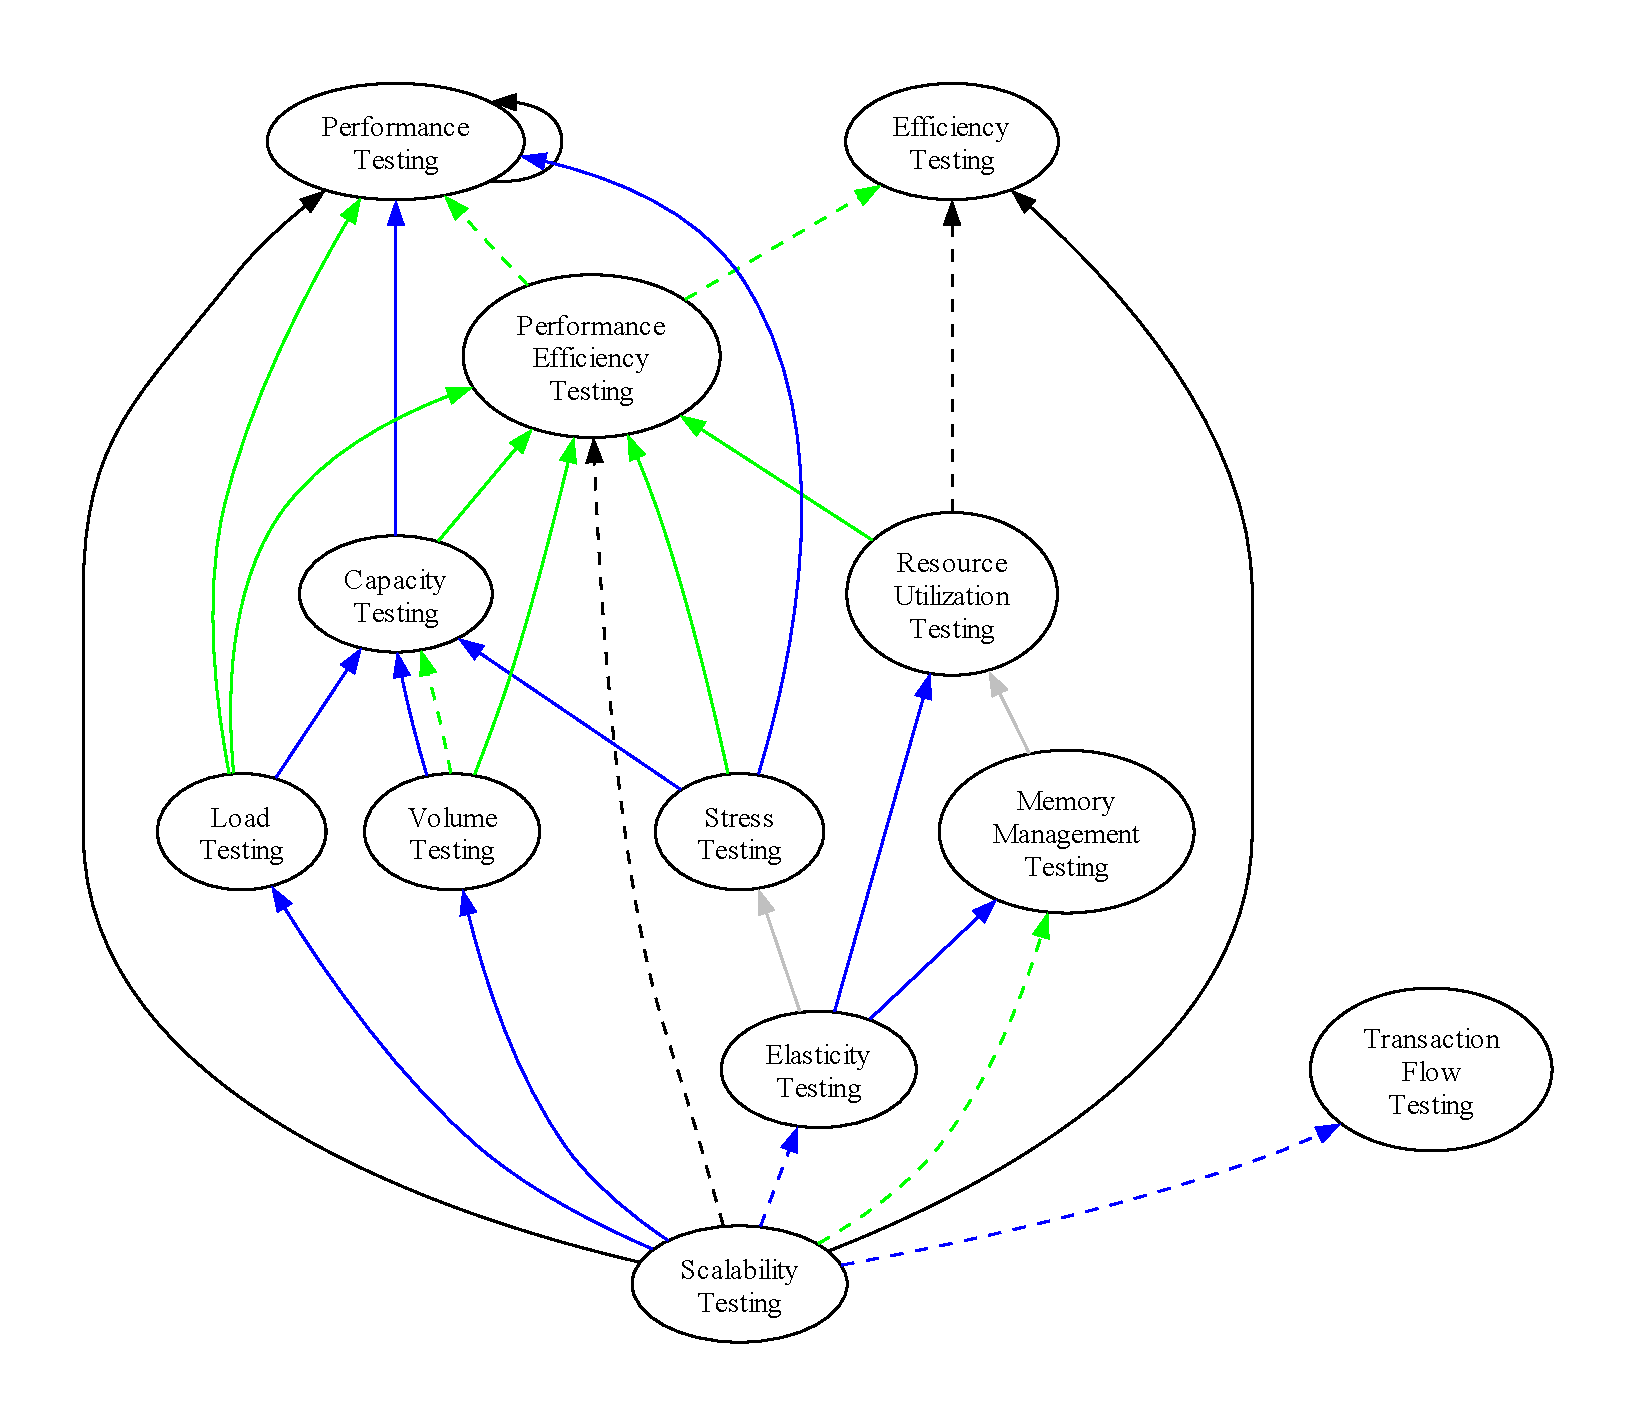
\includegraphics[width=\linewidth]{assets/graphs/scalabilityProposedGraph.pdf}
            \caption{Graph of proposed \ifnotpaper \else \\ \fi relations.}
            \label{fig:scal-graph-proposed}
        \end{subfigure}
        \caption{Graphs of relations between terms related to scalability testing.}
        \label{fig:scalGraphs}
    \end{figure}
}

\newcommand{\performanceGraph}{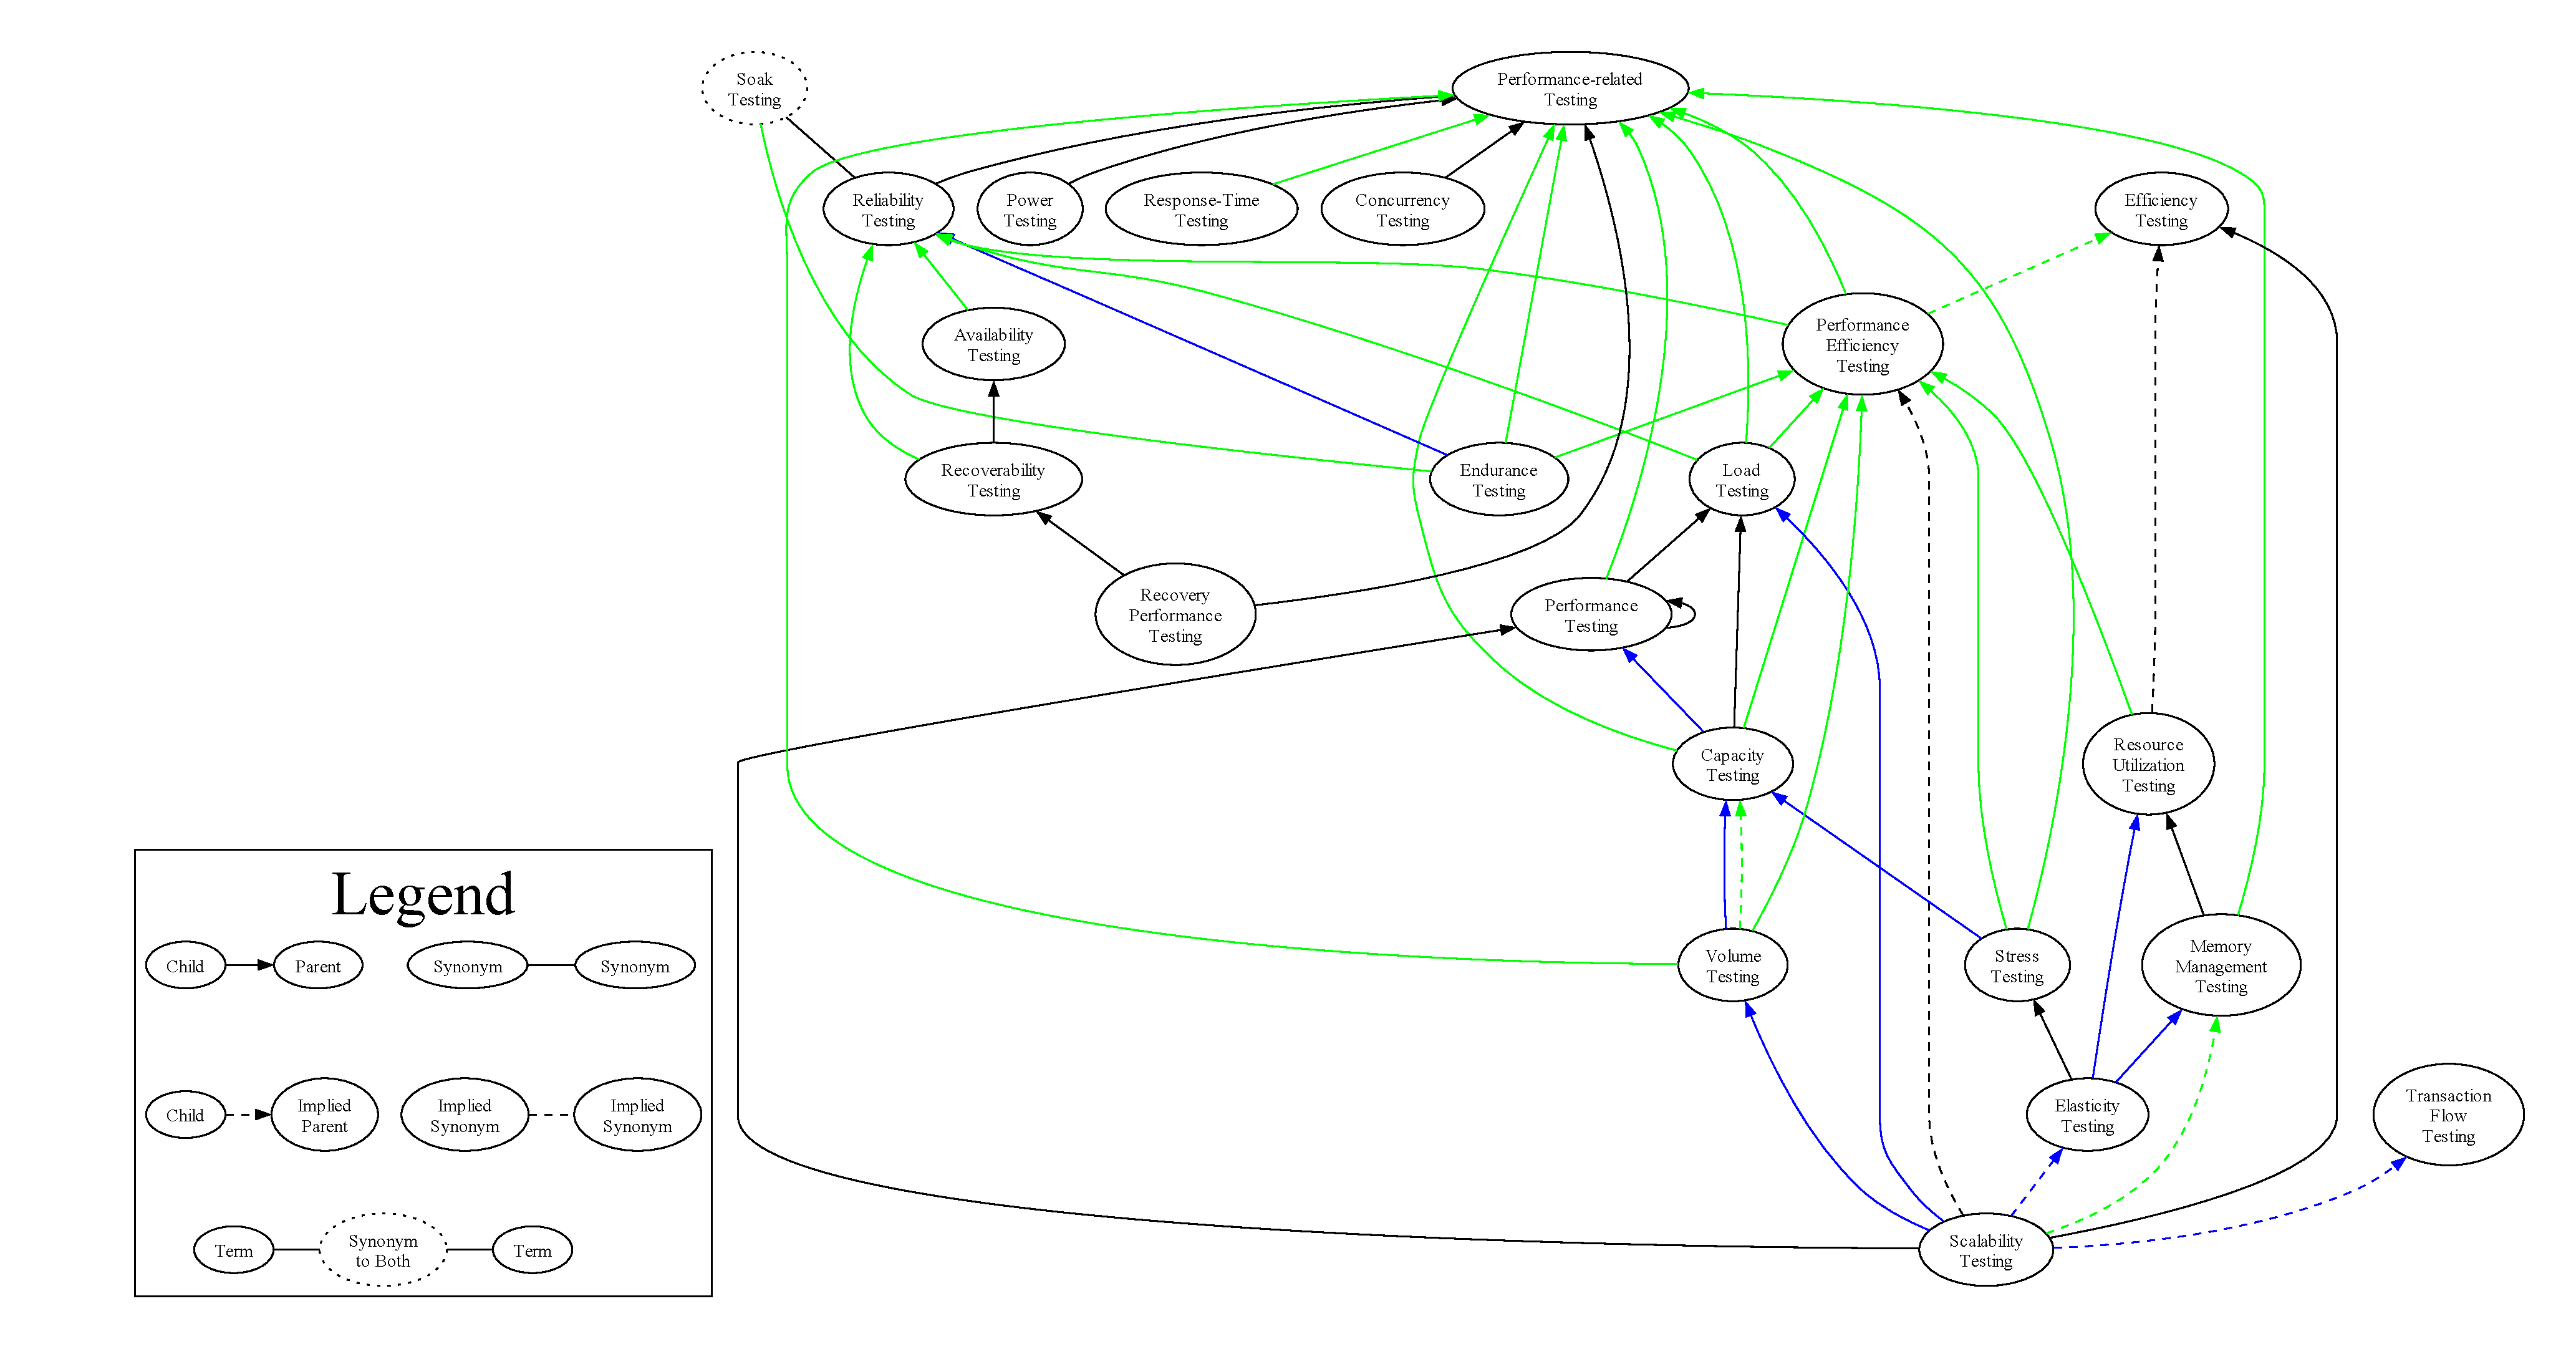
\includegraphics[width=\linewidth]{assets/graphs/performanceProposedGraph.pdf}}

%------------------------------------------------------------------------------
% Images & Figures
%------------------------------------------------------------------------------

\newcommand{\drasilLogo}{assets/images/drasil_logo.png}
\newcommand{\drasilLogoImg}{\begin{figure}[H]
    \centering
    \caption{Drasil's Logo}
    \label{fig:drasilLogo}

    \includegraphics[width=0.6\linewidth]{\drasilLogo}
\end{figure}
}
\newcommand{\refDrasilLogoImg}{\Cref{fig:drasilLogo}}

%------------------------------------------------------------------------------
% Tables
%------------------------------------------------------------------------------

% Organization of files
\newcommand{\organizationTable}{\begin{longtable}[c]{|>{\raggedright}p{0.3\linewidth}|>{\raggedright\arraybackslash}p{0.54\linewidth}|}
    \caption{Template Organization}
    \label{tab:organization}                                              \\

    \hline

    \rowcolor{McMasterMediumGrey}
    \textbf{File/Folder}     & \textbf{Intended Usage \& Description}
    \\ \hline

    \texttt{thesis.tex} & Focal \LaTeX{} file that collects everything and is
    used to build your thesis/report document.
    \\ \hline

    \texttt{Makefile} & A basic \texttt{Makefile} configuration. See
    \texttt{make help} for a list of helpful commands. \\ \hline

    \texttt{build/} & When you build your \acs{pdf}, this folder is used as the
    working directory of LuaLaTeX. Using this allows us to quickly get rid of
    \LaTeX{} build files that can cause problems when we re-build documents. \\
    \hline

    \texttt{manifest.tex} & Basic options that you should certainly configure
    according to your needs.
    \\ \hline

    \texttt{chapters.tex} & All chapters of your thesis should be included here.
    \\ \hline

    \texttt{chapters/} & Enumeration of the chapters of your thesis. I prefer
    using a two-digit indexing pattern for the prefix of file names so that I
    can quickly open up by chapter number using VS Codium. \\ \hline

    \texttt{assets.tex} & Enumeration of the various kinds of ``assets'' in the
    \texttt{assets/} folder. See the file for examples on how you can write your
    extra utility macros. \\ \hline

    \texttt{assets/} & Enumeration of various kinds of ``assets,'' with
    subdirectories for images and figures, tables, and code snippets. \\ \hline

    \texttt{front.tex} & All front matter of your thesis should be included
    here. \\ \hline

    \texttt{front/} & Enumeration of the front chapters of your thesis. These
    chapters should all be numbered using Roman numerals. \\ \hline

    \texttt{back.tex} & All back matter of your thesis should be included here.
    \\ \hline

    \texttt{back/} & Enumeration of the back matter content.
    \\ \hline

    \texttt{acronyms.tex} & List of acronyms you intend to use in your thesis.
    This uses the ``acro'' \LaTeX{} package.
    \\ \hline

    \texttt{macros.tex} & Helpful macros!
    \\ \hline

    \texttt{unicode\_chars.tex} & At times, you might find issues with unicode
    characters, especially in verbatim environments, where you might need to
    manually define them using other font glyphs.
    \\ \hline

    \texttt{mcmaster\_colours.tex} & Macros for the McMaster colour palette.
    \\ \hline

    \texttt{README.md} & Read it!
    \\ \hline

    \texttt{.gitignore} & List of files in the working directory that should be
    ignored by git.
    \\ \hline

    \texttt{latexmkrc} & Used for setting the timezone for latexmk, but can be
    used for other options.
    \\ \hline
\end{longtable}
}

\newcommand{\ieeeCatsTable}{% Conversion to longtblr assisted by GitHub Copilot

\begin{longtblr}[
    note{a} = {Also called ``test phase'' \ifnotpaper (see
            \discrepref{level-phase-syns}) \fi or ``test stage'' \ifnotpaper
            (see \discrepref{stage-level-syns})\else (see relevant synonym
            discrepancies in \Cref{syns})\fi.},
    note{b} = {Also called ``test design technique'' \ifnotpaper
            (\citealp[p.~11]{IEEE2022}; \citealpISTQB{})\else
            \cite[p.~11]{IEEE2022}, \cite{ISTQB}\fi.},
    caption={Categories of testing given by ISO/IEC and IEEE.},
    label={tab:ieeeCats}
    ]{
    colspec={|X[0.09,c,m]X[0.56,m]X[0.3,m]|},
    width = \linewidth, rowhead = 1, hlines
    }
    \thead{Term}                   & \thead{Definition}                           & \thead{Examples} \\
    Test Approach                  & A ``high-level test implementation choice''
    that includes ``test level, test type, test technique, test practice and
    \dots{} static testing'' \citep[p.~10]{IEEE2022} and is used to ``pick the
    particular test case values''
    \citeyearpar[p.~465]{IEEE2017} & black or white box, minimum and maximum
    boundary value testing \citep[p.~465]{IEEE2017}                                                  \\

    Test Level\TblrNote{a}         & A stage of testing ``typically associated
    with the achievement of particular objectives and used to treat particular
    risks'', each performed in sequence \ifnotpaper (\citealp[p.~12]{IEEE2022};
    \citeyear[p.~6]{IEEE2021}) \else \cite[p.~12]{IEEE2022}, \cite[p.~6]{IEEE2021}
    \fi with their ``own documentation and resources''
    \citeyearpar[p.~469]{IEEE2017} % ; more generally, ``designat[es] \dots\ the
    % coverage and detail'' \citeyearpar[p.~249]{IEEE2017} 
                                   & unit/component testing, integration testing,
    system testing, acceptance testing \ifnotpaper (\citealp[p.~12]{IEEE2022};
    \citeyear[p.~6]{IEEE2021}; \citeyear[p.~467]{IEEE2017}) \else
    \cite[p.~12]{IEEE2022}, \cite[p.~467]{IEEE2017}, \cite[p.~6]{IEEE2021} \fi                       \\
    Test Practice                  & A ``conceptual framework that can be
    applied to \dots{} [a] test process to facilitate testing'' \ifnotpaper
    (\citealp[p.~14]{IEEE2022}; \citeyear[p.~471]{IEEE2017}; OG IEEE 2013)
    \else \cite[p.~14]{IEEE2022}, \cite[p.~471]{IEEE2017}
    \fi % ; more generally, a ``specific type of activity that contributes to
    % the execution of a process'' \citeyearpar[p.~331]{IEEE2017} 
                                   & scripted testing, exploratory testing,
    automated testing \citep[p.~20]{IEEE2022}                                                        \\
    Test Technique\TblrNote{b}     & A ``procedure used to create or select a
    test model, identify test coverage items, and derive corresponding test
    cases'' \ifnotpaper (\citeyear[p.~11]{IEEE2022}; similar in
    \citeyear[p.~467]{IEEE2017}) \else \cite[p.~11]{IEEE2022} (similar in
    \cite[p.~467]{IEEE2017}) \fi that ``generate evidence that test item
    requirements have been met or that defects are present in a test item''
    \citeyearpar[p.~vii]{IEEE2021} % ; ``a variety \dots\ is typically
    % required to suitably cover any system'' \citeyearpar[p.~33]{IEEE2022} and
    % is ``often selected based on team skills and familiarity, on the format
    % of the test basis'', and on expectations \citeyearpar[p.~23]{IEEE2022}
                                   & equivalence partitioning,
    boundary value analysis, branch testing \citep[p.~11]{IEEE2022}                                  \\
    Test Type                      & ``Testing that is focused on specific
    quality characteristics'' \ifnotpaper (\citealp[p.~15]{IEEE2022};
    \citeyear[p.~7]{IEEE2021}; \citeyear[p.~473]{IEEE2017}; OG IEEE 2013)
    \else \cite[p.~15]{IEEE2022}, \cite[p.~473]{IEEE2017}, \cite[p.~7]{IEEE2021}
    \fi                            & security testing, usability testing,
    performance testing \ifnotpaper (\citealp[p.~15]{IEEE2022};
    \citeyear[p.~473]{IEEE2017}) \else\cite[p.~15]{IEEE2022},
    \cite[p.~473]{IEEE2017} \fi                                                                      \\
\end{longtblr}
}
\newcommand{\otherCatsTable}{% Defined here so VS Code doesn't freak out
\def\ieeeEquiv{\makecell{IEEE\\Equivalent}}
\def\swebokLevel{{Level\\(objective-\\based)\TblrNote{a}}}

\begin{longtblr}[
    note{a} = {See \flawref{stage-level-syns}.},
    note{b} = {Testing methods and guidances are omitted from this table
            since \citet{BarbosaEtAl2006} do not define or give examples of them.},
    note{c} = {Synonyms for these examples are used by
            \citet[p.~3; OG Mathur, 2012]{SouzaEtAl2017} and
            \citet[p.~3]{BarbosaEtAl2006}.},
    caption={Categories of testing given by other sources.},
    label={tab:otherCats}
    ]{
    colspec={|X[0.08,c,m]|X[0.43,m]|X[0.34,m]|Q[c,m]|},
    width = \linewidth, rowhead = 1
    }
    \hline
    \thead{Term}                           & \thead{Definition}           & \thead{Examples} & \thead{\ieeeEquiv{}} \\
    \hline
    % Guidance                               & none given
    % \citep[p.~3]{BarbosaEtAl2006}          & none given         & Technique?                              \\
    \swebokLevel{}                         & Test levels based on the
    purpose of testing \citep[p.~5\=/6]{SWEBOK2024} that ``determine
    how the test suite is identified \dots\ regarding its consistency
    \dots\ and its composition''
    \citetext{p.~5\=/2}                    & conformance testing,
    installation testing, regression testing, performance testing,
    security testing % reliability testing,
    \citep[pp.~5\=/7 to 5\=/9]{SWEBOK2024} & Type?                                                                  \\
    % Method                                 & none given
    % \citep[p.~3]{BarbosaEtAl2006}          & none given         & Practice?                               \\
    Phase                                  & none given
    %(\citealp[p.~221]{Perry2006}; \citealp[p.~3]{BarbosaEtAl2006})  
                                           & unit testing,
    integration testing, system testing, regression testing (\citealp[p.~221]{Perry2006};
    \citealp[p.~3]{BarbosaEtAl2006})       & Level                                                                  \\
    Procedure                              & The basis for how
    testing is performed that guides the process; ``categorized in[to] testing methods,
    testing guidances\TblrNote{b} and testing techniques''
    \citep[p.~3]{BarbosaEtAl2006}          & none given
    generally; see ``Technique''           & Approach                                                               \\
    Process                                & ``A sequence of
    testing steps'' \citep[p.~2]{BarbosaEtAl2006} ``based on a development technology and \dots\
    paradigm, as well as on a testing procedure''
    \citetext{p.~3}                        & none given                   & Practice                                \\
    Stage                                  & An
    alternative to the ``traditional \dots\ test stages'' %\footnote{See ``Level'' in \Cref{tab:ieeeCats}.}
    based on ``clear technical groupings''
    \citep[p.~13]{Gerrard2000a}            & desktop development testing,
    infrastructure testing,
    % system testing, large scale integration, and
    post-deployment monitoring
    \citep[p.~13]{Gerrard2000a}            & Level                                                                  \\
    Technique                              & ``Systematic
    procedures and approaches for generating or selecting the most suitable test suites''
    \citep[p.~5\=/10]{SWEBOK2024}          & specification-based testing,
    % ``on a sound theoretical basis'' \citep[p.~3]{BarbosaEtAl2006}
    structure-based testing, fault-based testing\TblrNote{c}
    % , experience-based testing, usage-based testing
    (\citealp[pp.~5\=/10, 5\=/13 to 5\=/15]{SWEBOK2024})
    % black-box, white-box, defect/fault-based, model-based testing
    % \citetext{\citealp[p.~3]{SouzaEtAl2017}; OG Mathur, 2012};
    % functional, structural, error-based, state-based testing \citep[p.~3]{BarbosaEtAl2006}
                                           & Technique                                                              \\
    \hline
\end{longtblr}
}
\newcommand{\otherCategorizationsTable}{\def\selecExs{Deterministic Testing\\ Random Testing}
\def\covExs{Input Space Partitioning\\ Graph Coverage\\ Logic Coverage\\ Syntax-based Testing}
\def\execExs{Static Testing\\ Dynamic Testing}
\def\goalExs{Verification Testing\\ Validation Testing}
\def\propExs{Functional Testing\\ Non-functional Testing}

\begin{paperTable}
    \centering
    \begin{minipage}{\linewidth}
        \begin{longtblr}[
            note{\textrm{a}} = {We also consider this categorization meaningful (see \Cref{static-test}).},
            note{\textrm{b}} = {Functional testing is categorized ambiguously (see \Cref{func-test-discrep}) and non-functional testing is uncategorized.},
            caption = {Alternate categorizations given by the literature.},
            label = {tab:otherCategorizations}
            ]{
            colspec = {|X[0.35,c,m]X[0.2,c,m]X[0.35,c,m]|}, width = \linewidth,
            rowhead = 1
            }
            \hline
            \thead{Test Basis}                                        & \thead{Example Approaches} & \thead{Subset of}                                                                                                                      \\
            \hline
            Selection Process \citep[p.~5-16]{SWEBOK2024}             & \selecExs{}                & Technique \citep[pp.~5-12, 5-16]{SWEBOK2024}                                                                                           \\
            \hline
            Coverage Criteria \citep[pp.~18--19]{AmmannAndOffutt2017} & \covExs{}                  & Technique (\citealp[p.~22]{IEEE2022}; \citeyear[Fig.~2]{IEEE2021}; \citealp[p.~5-11]{SWEBOK2024}; \citealp[pp.~47--48]{Firesmith2015}) \\
            \hline
            Execution of Code{\MidTblrNote{\textrm{a}}} (\citealp[p.~214]{KuļešovsEtAl2013}; \citealp[p.~12]{Gerrard2000a};
            \citealp[p.~53]{Patton2006})                              & \execExs{}                 & Approach                                                                                                                               \\
            \hline
            Goal of Testing (\citealp[p.~214]{KuļešovsEtAl2013};
            \citealp[pp.~69--70]{Perry2006})                          & \goalExs{}                 & Approach                                                                                                                               \\
            \hline
            Property of Code \citep[p.~213]{KuļešovsEtAl2013}
            or Test Target \citep[pp.~4--5]{Kam2008}                  & \propExs{}                 & Approach\TblrNote{\textrm{b}}                                                                                                          \\
            \hline
        \end{longtblr}
    \end{minipage}
\end{paperTable}
}

\newcommand{\sntxFlawsTable}{\begin{paperTable}
    \centering
    \caption{Breakdown of identified \nameref{sntxFlaws} by \srcCat{}.}
    \label{tab:sntxFlaws}
    \begin{minipage}{\linewidth}
        \begin{tabular}{|r|*{6}{cc|}c|}
            \hline
                              & \multicolumn{2}{c|}{\thead{\nameref{wrong}}} & \multicolumn{2}{c|}{\thead{\nameref{miss}}} & \multicolumn{2}{c|}{\thead{\nameref{contra}}} & \multicolumn{2}{c|}{\thead{\nameref{ambi}}} & \multicolumn{2}{c|}{\thead{\nameref{over}}} & \multicolumn{2}{c|}{\thead{\reduns{}}} &                                                                                                                                                                                         \\
            \thead{\srcCat{}} & \thead{Exp}                                  & \thead{Imp}                                 & \thead{Exp}                                   & \thead{Imp}                                 & \thead{Exp}                                 & \thead{Imp}                            & \thead{Exp}             & \thead{Imp}             & \thead{Exp}             & \thead{Imp}              & \thead{Exp}              & \thead{Imp}              & \thead{Total}            \\
            \hline
            \stds{}           & \stdSntxFlawBrkdwn{1}                        & \stdSntxFlawBrkdwn{2}                       & \stdSntxFlawBrkdwn{3}                         & \stdSntxFlawBrkdwn{4}                       & \stdSntxFlawBrkdwn{5}                       & \stdSntxFlawBrkdwn{6}                  & \stdSntxFlawBrkdwn{7}   & \stdSntxFlawBrkdwn{8}   & \stdSntxFlawBrkdwn{9}   & \stdSntxFlawBrkdwn{10}   & \stdSntxFlawBrkdwn{11}   & \stdSntxFlawBrkdwn{12}   & \stdSntxFlawBrkdwn{13}   \\
            \metas{}          & \metaSntxFlawBrkdwn{1}                       & \metaSntxFlawBrkdwn{2}                      & \metaSntxFlawBrkdwn{3}                        & \metaSntxFlawBrkdwn{4}                      & \metaSntxFlawBrkdwn{5}                      & \metaSntxFlawBrkdwn{6}                 & \metaSntxFlawBrkdwn{7}  & \metaSntxFlawBrkdwn{8}  & \metaSntxFlawBrkdwn{9}  & \metaSntxFlawBrkdwn{10}  & \metaSntxFlawBrkdwn{11}  & \metaSntxFlawBrkdwn{12}  & \metaSntxFlawBrkdwn{13}  \\
            \texts{}          & \textSntxFlawBrkdwn{1}                       & \textSntxFlawBrkdwn{2}                      & \textSntxFlawBrkdwn{3}                        & \textSntxFlawBrkdwn{4}                      & \textSntxFlawBrkdwn{5}                      & \textSntxFlawBrkdwn{6}                 & \textSntxFlawBrkdwn{7}  & \textSntxFlawBrkdwn{8}  & \textSntxFlawBrkdwn{9}  & \textSntxFlawBrkdwn{10}  & \textSntxFlawBrkdwn{11}  & \textSntxFlawBrkdwn{12}  & \textSntxFlawBrkdwn{13}  \\
            \papersTbl{}      & \paperSntxFlawBrkdwn{1}                      & \paperSntxFlawBrkdwn{2}                     & \paperSntxFlawBrkdwn{3}                       & \paperSntxFlawBrkdwn{4}                     & \paperSntxFlawBrkdwn{5}                     & \paperSntxFlawBrkdwn{6}                & \paperSntxFlawBrkdwn{7} & \paperSntxFlawBrkdwn{8} & \paperSntxFlawBrkdwn{9} & \paperSntxFlawBrkdwn{10} & \paperSntxFlawBrkdwn{11} & \paperSntxFlawBrkdwn{12} & \paperSntxFlawBrkdwn{13} \\
            \hline
            Total             & \totalSntxFlawBrkdwn{1}                      & \totalSntxFlawBrkdwn{2}                     & \totalSntxFlawBrkdwn{3}                       & \totalSntxFlawBrkdwn{4}                     & \totalSntxFlawBrkdwn{5}                     & \totalSntxFlawBrkdwn{6}                & \totalSntxFlawBrkdwn{7} & \totalSntxFlawBrkdwn{8} & \totalSntxFlawBrkdwn{9} & \totalSntxFlawBrkdwn{10} & \totalSntxFlawBrkdwn{11} & \totalSntxFlawBrkdwn{12} & \totalSntxFlawBrkdwn{13} \\
            \hline
        \end{tabular}
    \end{minipage}
\end{paperTable}
}
\newcommand{\smntcFlawsTable}{\begin{paperTable}
    \centering
    \caption{Breakdown of identified \nameref{smntcFlaws} by \srcCat{}.}
    \label{tab:smntcFlaws}
    % \begin{minipage}{\linewidth}
    \begin{tabular}{|r|*{6}{cc|}c|}
        \hline
                          & \multicolumn{2}{c|}{\thead{\cats{}}} & \multicolumn{2}{c|}{\thead{\syns{}}} & \multicolumn{2}{c|}{\thead{\pars{}}} & \multicolumn{2}{c|}{\thead{\defs{}}} & \multicolumn{2}{c|}{\thead{\terms{}}} & \multicolumn{2}{c|}{\thead{\cites{}}} &                                                                                                                                                                                                \\
        % \cline{2-10}
        \thead{\srcCat{}} & \thead{Exp}                          & \thead{Imp}                          & \thead{Exp}                          & \thead{Imp}                          & \thead{Exp}                           & \thead{Imp}                           & \thead{Exp}              & \thead{Imp}              & \thead{Exp}              & \thead{Imp}               & \thead{Exp}               & \thead{Imp}               & \thead{Total}             \\
        \hline
        \stds{}           & \stdSmntcFlawBrkdwn{1}               & \stdSmntcFlawBrkdwn{2}               & \stdSmntcFlawBrkdwn{3}               & \stdSmntcFlawBrkdwn{4}               & \stdSmntcFlawBrkdwn{5}                & \stdSmntcFlawBrkdwn{6}                & \stdSmntcFlawBrkdwn{7}   & \stdSmntcFlawBrkdwn{8}   & \stdSmntcFlawBrkdwn{9}   & \stdSmntcFlawBrkdwn{10}   & \stdSmntcFlawBrkdwn{11}   & \stdSmntcFlawBrkdwn{12}   & \stdSmntcFlawBrkdwn{13}   \\
        \metas{}          & \metaSmntcFlawBrkdwn{1}              & \metaSmntcFlawBrkdwn{2}              & \metaSmntcFlawBrkdwn{3}              & \metaSmntcFlawBrkdwn{4}              & \metaSmntcFlawBrkdwn{5}               & \metaSmntcFlawBrkdwn{6}               & \metaSmntcFlawBrkdwn{7}  & \metaSmntcFlawBrkdwn{8}  & \metaSmntcFlawBrkdwn{9}  & \metaSmntcFlawBrkdwn{10}  & \metaSmntcFlawBrkdwn{11}  & \metaSmntcFlawBrkdwn{12}  & \metaSmntcFlawBrkdwn{13}  \\
        \texts{}          & \textSmntcFlawBrkdwn{1}              & \textSmntcFlawBrkdwn{2}              & \textSmntcFlawBrkdwn{3}              & \textSmntcFlawBrkdwn{4}              & \textSmntcFlawBrkdwn{5}               & \textSmntcFlawBrkdwn{6}               & \textSmntcFlawBrkdwn{7}  & \textSmntcFlawBrkdwn{8}  & \textSmntcFlawBrkdwn{9}  & \textSmntcFlawBrkdwn{10}  & \textSmntcFlawBrkdwn{11}  & \textSmntcFlawBrkdwn{12}  & \textSmntcFlawBrkdwn{13}  \\
        \papersTbl{}      & \paperSmntcFlawBrkdwn{1}             & \paperSmntcFlawBrkdwn{2}             & \paperSmntcFlawBrkdwn{3}             & \paperSmntcFlawBrkdwn{4}             & \paperSmntcFlawBrkdwn{5}              & \paperSmntcFlawBrkdwn{6}              & \paperSmntcFlawBrkdwn{7} & \paperSmntcFlawBrkdwn{8} & \paperSmntcFlawBrkdwn{9} & \paperSmntcFlawBrkdwn{10} & \paperSmntcFlawBrkdwn{11} & \paperSmntcFlawBrkdwn{12} & \paperSmntcFlawBrkdwn{13} \\
        \hline
        Total             & \totalSmntcFlawBrkdwn{1}             & \totalSmntcFlawBrkdwn{2}             & \totalSmntcFlawBrkdwn{3}             & \totalSmntcFlawBrkdwn{4}             & \totalSmntcFlawBrkdwn{5}              & \totalSmntcFlawBrkdwn{6}              & \totalSmntcFlawBrkdwn{7} & \totalSmntcFlawBrkdwn{8} & \totalSmntcFlawBrkdwn{9} & \totalSmntcFlawBrkdwn{10} & \totalSmntcFlawBrkdwn{11} & \totalSmntcFlawBrkdwn{12} & \totalSmntcFlawBrkdwn{13} \\
        \hline
    \end{tabular}
    % \end{minipage}
\end{paperTable}}

\newcommand{\testReqsTable}{% To prevent VSCode from aligning things weirdly
\def\typeHead{Testing\\Approach}

\begin{table}[hbtp!]
    \centering
    \caption{Testing Requirements}
    \label{tab:testReqs}
    \begin{tabularx}{\textwidth}{|p{0.14\textwidth}|X|c|c|}
        \hline
        \rowcolor{McMasterMediumGrey}
        \thead{\typeHead}       & \thead{Requirements}                         & \thead{In Drasil?} & \thead{Addable?} \\
        \hline
        Unit testing            & Code modules and their specifications        & ??                 & ??               \\
        Integration testing     & Code modules and their interfaces            & ??                 & ??               \\
        System testing          & Requirements specification; most of the code
                                & ??                                           & ??                                    \\
        Acceptance testing      & Customer requirements and feedback           & ??                 & ??               \\
        Installation testing    & Algorithm for installation; environments to
        test in; method to check
        successful installation & ??                                           & ??                                    \\
        \hline
    \end{tabularx}
\end{table}}


% Extra functionality for command parsing and commentary
\usepackage{xparse}
\usepackage{comment}

% Make \today only show month and year
\usepackage[en-CA]{datetime2}
\DTMlangsetup[en-CA]{showdayofmonth=false}

% Manifest data
%------------------------------------------------------------------------------
% Your Information
%------------------------------------------------------------------------------

\newcommand{\thesisType}{Thesis}

\newcommand{\thesisTitle}{My Thesis Title}
\newcommand{\thesisHalfTitle}{\thesisTitle}

\newcommand{\thesisAuthorName}{Johnny Appleseed}
\newcommand{\thesisAuthorNameShort}{J.\ Appleseed}
\newcommand{\thesisAuthorCredentials}{B.Sc.}
\newcommand{\thesisSupervisor}{Dr.\ Supervisor}

\newcommand{\thesisTargetDegreeNameShort}{M.Sc.}
\newcommand{\thesisTargetDegreeName}{Master of Science}

\newcommand{\thesisTargetDegreeFocus}{Computer Science}
\newcommand{\thesisTargetDegree}{\thesisTargetDegreeName{} in \thesisTargetDegreeFocus{}}

\newcommand{\thesisInstitutionDepartmentShort}{Computing and Software}
\newcommand{\thesisInstitutionGraduateStudies}{School of Graduate Studies}
\newcommand{\thesisInstitutionDepartment}{Department of \thesisInstitutionDepartmentShort{}}
\newcommand{\thesisInstitution}{McMaster University}
\newcommand{\thesisCityProvince}{Hamilton, Ontario}

\newcommand{\thesisSubmissionYear}{\the\year{}}
\newcommand{\thesisSubmissionMonthYear}{\DTMtoday{}}

%------------------------------------------------------------------------------
% Metadata
%------------------------------------------------------------------------------

% The label placed on the last page of the front matter is used to find how many
% pages belong in the front matter (which are numbered with roman numerals
% instead of the traditional arabic numbering system). You only need to update
% this label value IF the "Declaration of Academic Achievement" is not the last
% page of your front matter.
\newcommand{\thesisLastPageOfFrontMatterLabel}{chap:declaration_of_academic_achievement}

%------------------------------------------------------------------------------
% Options
%------------------------------------------------------------------------------

% - COMPILE FOR PRINTING THE PDF                              (default = false)
%   If enabled, 'porthref'* links will appear in footnotes to assist readers.
\newif\ifcompilingforprinting
% \compilingforprintingtrue % Enable
\compilingforprintingfalse % Disable

% - DOUBLE SPACING                                            (default = 2x)
% \newcommand{\thesisSpacing}{\doublespacing}
% \newcommand{\thesisSpacing}{\singlespacing}
\newcommand{\thesisSpacing}{\linespread{1}}

% - QUESTION-DIRECTED WRITING & TO-DOS SWITCH                 (default = true)
%   If enabled, "writing directive" boxes will be displayed in the PDF
\newif\ifshowwritingdirectives
\showwritingdirectivestrue % Show questions and to-do notes
% \showwritingdirectivesfalse % Don't show questions and to-do notes

% - RESET FOOTNOTE NUMBERING FOR EACH PAGE                    (default = false)
%   If enabled, the footnote numbering will reset to 1 on each new page
\newif\ifresetfootnotecounter
% \resetfootnotecountertrue % Reset footnote numbering on each page
\resetfootnotecounterfalse % Don't reset footnote numbering on each page

% - MARGIN SIZES
\newcommand{\thesisMarginTop}{3.8cm}                        % ("official" = 3.8cm)
\newcommand{\thesisMarginBottom}{2.5cm}                     % ("official" = 2.5cm)
\newcommand{\thesisMarginInner}{3.8cm}                      % ("official" = 3.8cm, recommended = 2.5cm)
\newcommand{\thesisMarginOuter}{2.5cm}                      % ("official" = 2.5cm)
\newcommand{\thesisMarginHeadheight}{15pt}                  % (default = 15pt)
\newcommand{\thesisTODOMarginSize}{3.5cm}                   % (default = 3.5cm, recommended = 2.25cm)


% Configure font and file encodings, and language as Canadian English
\usepackage{fontspec}
\usepackage[canadian]{babel}
\usepackage{lmodern}
\usepackage{anyfontsize}

% Math-related, but also generally helpful
\usepackage{proof}
\usepackage{amsthm}
\usepackage{mathrsfs}
\usepackage[pdf]{graphviz}
\usepackage{longtable}
\usepackage{svg}
\usepackage{mathpartir}
\usepackage{braket}

% Since LaTeX doesn't, and many fonts rarely, fully support unicode, we need to
% manually create characters to replace missing glyphs.
\usepackage{newunicodechar}
% At times, if you use raw unicode characters, you'll come across the following error:
% Missing character: There is no • (U+2022) in font ec-lmtt12!

% More, generally,
% Missing character: There is no `X` (U+`Y`) in font `Z`!

% To solve this  issue, we may manually replace instances of them with re-built
% copies of them. They may look a bit out of place because they don't follow the
% same font, but you can make them look decent if you replace them with simpler
% variants within the font. Try your best!

% For example, to resolve the above issue, we may use:
% \newunicodechar{•}{\(\cdot{}\)}

\newunicodechar{•}{\(\cdot{}\)}
\newunicodechar{‘}{\textquoteleft{}}
\newunicodechar{’}{\textquoteright{}}
\newunicodechar{≠}{\(\neq\)}


% Tiny package for easily grabbing the page count of the "main matter"
\usepackage{lastpage}

% For quotes, I wanted to put the "left bar" style. For implementation, Gonzalo
% Medina was very kind to create an example. It is based on:
% https://tex.stackexchange.com/a/50623
\usepackage{framed}
\usepackage[framemethod=TikZ]{mdframed}
\newmdenv[topline=false, rightline=false, bottomline=false,%
    linewidth=2pt, innerrightmargin=0pt, leftmargin=0pt,%
    innerleftmargin=5pt, skipabove=8pt, skipbelow=8pt]{mdleftbar}

\newmdenv[linewidth=2pt, linecolor=green, backgroundcolor=green!8, roundcorner=10pt,
    skipabove=8pt, skipbelow=8pt]{mdwritingdirectives}

% For nice captions and floating environments, such as for my code snippets
\usepackage{caption}
\usepackage{float}

% For inline-able list environments
\usepackage{paralist}

% Extra features for changing page widths ("adjustwidth" is a helpful environment!)
\usepackage{changepage}

% For code highlighting
\usepackage[newfloat,outputdir=build]{minted}
% Credits to Arash Esbati (https://tex.stackexchange.com/a/254177) for the
% listings-related component of minted usage.

\usemintedstyle{colorful}

% Configure page shape
\usepackage[
    a4paper,
    top=\thesisMarginTop{},
    bottom=\thesisMarginBottom{},
    inner=\thesisMarginInner{},
    outer=\thesisMarginOuter{},
    headheight=\thesisMarginHeadheight{},
]{geometry}

\usepackage{afterpage}

% Allow labelling enum items: Credits to: https://texblog.org/2012/03/21/cross-referencing-list-items/
\usepackage{enumitem}
\makeatletter
\def\namedlabel#1#2{\begingroup
    \textbf{#2}%
    \def\@currentlabel{#2}%
    \phantomsection\label{#1}\endgroup
}
\makeatother

\ifresetfootnotecounter
    % Make footnote counter reset for each new page.
    \usepackage{footnpag}
\fi

% Set spacing according to manifest
\usepackage{setspace}
\thesisSpacing{}

% Required for biblatex, but also adds functionality for quotation
\usepackage{csquotes}

% Jason's bibliography format
% % Credit to Gabriel Devenyi for this bibliography cfg:
% % github.com/gdevenyi/mcmaster.latex
% \usepackage[
%   style=numeric-comp,
%   backend=biber,
%   sorting=none,
%   backref=true,
%   maxnames=99,
%   alldates=iso,
%   seconds=true
% ]{biblatex} % bibliography
% \addbibresource{references.bib}
\usepackage[round]{natbib}
\bibliographystyle{plainnat}
\setcitestyle{yysep={;}}
\defcitealias{ISTQB}{Hamburg and Mogyorodi}
\newcommand{\citetISTQB}{\citetalias{ISTQB} (\citeyear{ISTQB})}
\newcommand{\citepISTQB}{\citepalias[\citeyear{ISTQB}]{ISTQB}}
\newcommand{\citealpISTQB}{\citetalias{ISTQB}, \citeyear{ISTQB}}

% Fancy Headers
\usepackage{fancyhdr}

% Allow more line breaks in URLs
\usepackage{xurl}

% Enable links within the document
\usepackage{hyperref}
\hypersetup{
    colorlinks=true,
    linkcolor=red,
    urlcolor=red,
    breaklinks=true,
    pdftitle={\thesisTitle{}},
    pdfauthor={\thesisAuthorName{}}
}
\urlstyle{rm} % Make URL styled fonts match hyperref's hrefs
\usepackage[nameinlink]{cleveref} % Fixes capitalization of internal references

\usepackage{array}

% For abbreviations, we use "acro" package, and mfirstuc to help capitalize long
% versions normally
\usepackage{mfirstuc}
\MFUhyphentrue % tell mfirstuc to capitalize hyphenated words

% General Utility Functions
%------------------------------------------------------------------------------
% Question-directed Writing
%------------------------------------------------------------------------------

\ifshowwritingdirectives
  \newenvironment{writingdirectives}{\begin{mdwritingdirectives}\centering\textbf{Writing Directives}\begin{itemize}}{\end{itemize}\end{mdwritingdirectives}}
\else
  \excludecomment{writingdirectives}
\fi

%------------------------------------------------------------------------------
% Spacing Options
%------------------------------------------------------------------------------

\newcommand{\thesisForceSingleSpacing}{\singlespacing}
\newcommand{\thesisForceDoubleSpacing}{\doublespacing}

%------------------------------------------------------------------------------
% Footnotes that only show when "compiling for printing."
%------------------------------------------------------------------------------

\ifcompilingforprinting
  \newcommand{\printOnlyFootnote}[1]{\footnote{#1}}
  \newcommand{\printOnlyFootnoteText}[1]{\footnotetext{#1}}
  \newcommand{\printOnlyFootnoteMark}{\footnotemark}
\else
  \newcommand{\printOnlyFootnote}[1]{}
  \newcommand{\printOnlyFootnoteText}[1]{}
  \newcommand{\printOnlyFootnoteMark}{}
\fi

%------------------------------------------------------------------------------
% Portable HREFs
%------------------------------------------------------------------------------

% Common variant
\newcommand{\porthref}[2]{\href{#2}{#1}\printOnlyFootnote{\url{#2}}}

% Custom URLs
\newcommand{\porthreft}[3]{\href{#3}{#1}\printOnlyFootnote{\href{#3}{#2}}}
% Inside of some environments, footnote marks aren't registered properly, so we
% need to manually write the "text" part
\newcommand{\porthreftm}[2]{\href{#2}{#1\printOnlyFootnoteMark}}

%------------------------------------------------------------------------------
% TODOs
%------------------------------------------------------------------------------

% Generic Inlined TODOs
\newcommand{\intodo}[1]{\todo[inline]{#1}}

% Unimportant TODOs for "later" (i.e., finishing touches or changes immediately before submission)
\newcommand{\latertodo}[1]{\todo[backgroundcolor=Cyan]{\textit{Later}: #1}}

% "Important" TODOs
\newcommand{\imptodo}[1]{\todo[inline,backgroundcolor=Red]{\textbf{Important}: #1}}

% "Easy" TODOs
\newcommand{\easytodo}[1]{\todo[inline,backgroundcolor=SeaGreen]{\textit{Easy}: #1}}
\newcommand{\eztodo}[1]{\easytodo{#1}}

% "Tedious" TODOs
\newcommand{\tedioustodo}[1]{\todo[inline,backgroundcolor=PineGreen]{\textit{Needs time}: #1}}

% "Question" TODO Notes
\newcounter{todonoteQuestionsCtr}
\newcommand{\questiontodo}[1]{\stepcounter{todonoteQuestionsCtr}\todo[backgroundcolor=Lavender]{\textbf{Q \#\thetodonoteQuestionsCtr{}}: #1}}
\newcommand{\qtodo}[1]{\questiontodo{#1}}

%------------------------------------------------------------------------------
% Code Snippets
%------------------------------------------------------------------------------

\newenvironment{code}{\captionsetup{type=listing,skip=14pt}}{}
\SetupFloatingEnvironment{listing}{name=Source Code, listname=List of Source Codes}
\crefname{listing}{source code}{source codes}
\Crefname{listing}{Source Code}{Source Codes}

\newenvironment{haskell}[3]
{\VerbatimEnvironment\thesisForceSingleSpacing{}\begin{code}\captionof{listing}[#1]{\protect\porthreftm{#1}{#3}}\printOnlyFootnoteText{\protect\url{#3}}\label{lst:#2}\begin{minted}[frame=lines,framerule=2pt,breaklines]{haskell}}
  {\end{minted}\end{code}\thesisSpacing{}}

\newenvironment{codeSnippet}[4]
{\VerbatimEnvironment\thesisForceSingleSpacing{}\begin{code}\captionof{listing}[#2]{\protect\porthreftm{#2}{#4}}\printOnlyFootnoteText{\protect\url{#4}}\label{lst:#3}\begin{minted}[frame=lines,framerule=2pt,breaklines]{#1}}
  {\end{minted}\end{code}\thesisSpacing{}}

\newenvironment{pseudohaskell}[2]
{\VerbatimEnvironment\thesisForceSingleSpacing{}\begin{code}\captionof{listing}{Pseudocode: #1}\label{lst:#2}\begin{minted}[frame=lines,framerule=2pt,breaklines]{haskell}}
  {\end{minted}\end{code}\thesisSpacing{}}

\newenvironment{pseudocode}[3]
{\VerbatimEnvironment\thesisForceSingleSpacing{}\begin{code}\captionof{listing}{Pseudocode: #2}\label{lst:#3}\begin{minted}[frame=lines,framerule=2pt,breaklines]{#1}}
  {\end{minted}\end{code}\thesisSpacing{}}

\newcommand{\inlineHs}[1]{\mintinline{haskell}|#1|}
\newcommand{\inlineCode}[2]{\mintinline{#1}|#2|}

%------------------------------------------------------------------------------
% Link to Drasil issue
%------------------------------------------------------------------------------

\newcommand{\issueref}[1]{\href{https://github.com/JacquesCarette/Drasil/issues/#1}{\##1}}
\newcommand{\pullref}[1]{\href{https://github.com/JacquesCarette/Drasil/pull/#1}{\##1}}
\newcommand{\thesisissueref}[1]{\href{https://github.com/samm82/TestGen-Thesis/issues/#1}{\##1}}


\notpapertrue

% For fancy pictures
\usepackage{tikz}
\usetikzlibrary{shapes,arrows,cd,babel,arrows.meta,graphs,graphdrawing}
\usegdlibrary {layered}

% Make sure the floating lists (figures, source codes, and abbreviations) are
% shown in the toc.
\usepackage{tocbibind}

% Counters
\usepackage{chngcntr}

\title{
{Software Testing Overview}\\
{\thesisInstitution{}}
}
\author{\thesisAuthorName{}}
\date{\thesisSubmissionMonthYear{}}

% START : TODO LIST SETUP
\ifshowwritingdirectives
    \usepackage[backgroundcolor=yellow,colorinlistoftodos]{todonotes}
    \setlength{\marginparwidth}{\thesisTODOMarginSize{}}
    \reversemarginpar % place on left-hand side
\else
    \usepackage[disable]{todonotes}
\fi
% END   : TODO LIST SETUP

% From https://tex.stackexchange.com/a/61803/192195
\newenvironment{leveldown}% Demote sectional commands
{\let\chapter\section%
    \let\section\subsection%
    \let\subsection\subsubsection%
    \let\subsubsection\paragraph%
    \let\paragraph\subparagraph%
    %\let\subparagraph\relax%
}{}
\newenvironment{levelup}% Promote sectional commands
{\let\subparagraph\paragraph%
    \let\paragraph\subsubsection%
    \let\subsubsection\subsection%
    \let\subsection\section%
    \let\section\chapter%
    %\let\chapter\relax%
}{}

\newenvironment{paperTable}{
    \begin{table}[hbtp!]
        }{
    \end{table}
}

\newenvironment{paperFigure}{
    \begin{figure}[hbtp!]
        }{
    \end{figure}
}